% GBFS Audit Catalogue --- Computer Standards & Interfaces submission draft
% Reformatted from the Patterns (Cell Press) draft (gold_standard_patterns.tex)
% for Elsevier Computer Standards & Interfaces author guidelines:
%   - <=250 word abstract
%   - 3-5 highlights, each <=85 characters
%   - 1-7 keywords
%   - numbered sections (1, 1.1, ...)
%   - numbered references [1] (style: unsrt)
%   - CRediT author contributions
%   - explicit declarations of interests / generative AI use
%   - data availability statement

\documentclass[11pt,a4paper]{article}

\usepackage[T1]{fontenc}
\usepackage[utf8]{inputenc}
\usepackage{lmodern}
\usepackage[margin=2.5cm]{geometry}
\usepackage{microtype}
\usepackage{amssymb,amsmath,amstext}
\usepackage{booktabs}
\usepackage{longtable}
\usepackage{graphicx}
\usepackage{adjustbox}
\graphicspath{{figures/}}
\usepackage{algorithm2e}
\usepackage{xcolor}
\usepackage{url}
\usepackage[colorlinks=true,linkcolor=blue,citecolor=blue,urlcolor=blue]{hyperref}
\usepackage{xr}
\externaldocument{supplementary}
\usepackage{enumitem}
\usepackage{caption}
\usepackage{titlesec}
\usepackage{authblk}

% Discourage widows/orphans (a single line stranded at the top/bottom of a page)
\widowpenalty=10000
\clubpenalty=10000

\titleformat{\section}{\large\bfseries\sffamily\color{black!85}}{\thesection}{0.8em}{}
\titleformat{\subsection}{\normalsize\bfseries\sffamily\color{black!75}}{\thesubsection}{0.8em}{}

\newcommand{\ie}{\emph{i.e.}}
\newcommand{\eg}{\emph{e.g.}}
\newcommand{\etc}{etc.}

% --- Anonymity toggle for double-blind submission ---
% Submission build is anonymous; set \anonymousfalse for the named camera-ready.
\newif\ifanonymous
\anonymoustrue
\newcommand{\zdoi}{\ifanonymous\texttt{[deposited on Zenodo; DOI withheld for review]}\else\texttt{10.5281/zenodo.20125460}\fi}
\newcommand{\codeurl}{\ifanonymous\texttt{[anonymised repository; link provided on acceptance]}\else\url{https://github.com/rohanfosse/gbfs-audit-catalogue}\fi}
\newcommand{\hfurl}{\ifanonymous\texttt{[anonymised dataset mirror]}\else\url{https://huggingface.co/datasets/rohanfosse/gbfs-audit-catalogue}\fi}
\newcommand{\toolkitdoi}{\ifanonymous\texttt{[reference-implementation library archived on Zenodo; DOI withheld for review]}\else\texttt{10.5281/zenodo.20992153}\fi}
\newcommand{\toolkiturl}{\ifanonymous\texttt{[anonymised library repository; link provided on acceptance]}\else\url{https://github.com/cycling-data-lab/gbfs-toolkit}\fi}

\newenvironment{highlights}{%
  \par\noindent\textsf{\bfseries\large Highlights}\par\smallskip
  \begin{itemize}[leftmargin=1.4em,itemsep=0.15em,topsep=0.2em]}{%
  \end{itemize}\par\medskip}

\title{\bfseries\sffamily\Large Auditing GBFS bike-sharing feeds:\\
a reproducible anomaly taxonomy for open mobility data,\\
validated in France and projected across 48 countries}

\ifanonymous
\author{Anonymous Author(s)}
\else
\author[1]{Rohan Foss\'e\thanks{Lead contact: \texttt{rfosse@cesi.fr}}}
\author[2]{Ga\"el Pallares}
\affil[1]{CESI Engineering School, Montpellier, France}
\affil[2]{CESI LINEACT (EA 7527), Montpellier, France}
\fi
\date{}

\begin{document}
\maketitle

% Graphical abstract: per Elsevier CSI author guidelines the graphical
% abstract is uploaded as a separate file via Editorial Manager and is
% NOT embedded in the manuscript PDF. The file `fig00_visual_abstract.png`
% in `figures/` is the production asset to upload at submission time.
% (Comment the block below in/out for working drafts vs. final submission.)
%
% \begin{figure}[!t]
% \centering
% 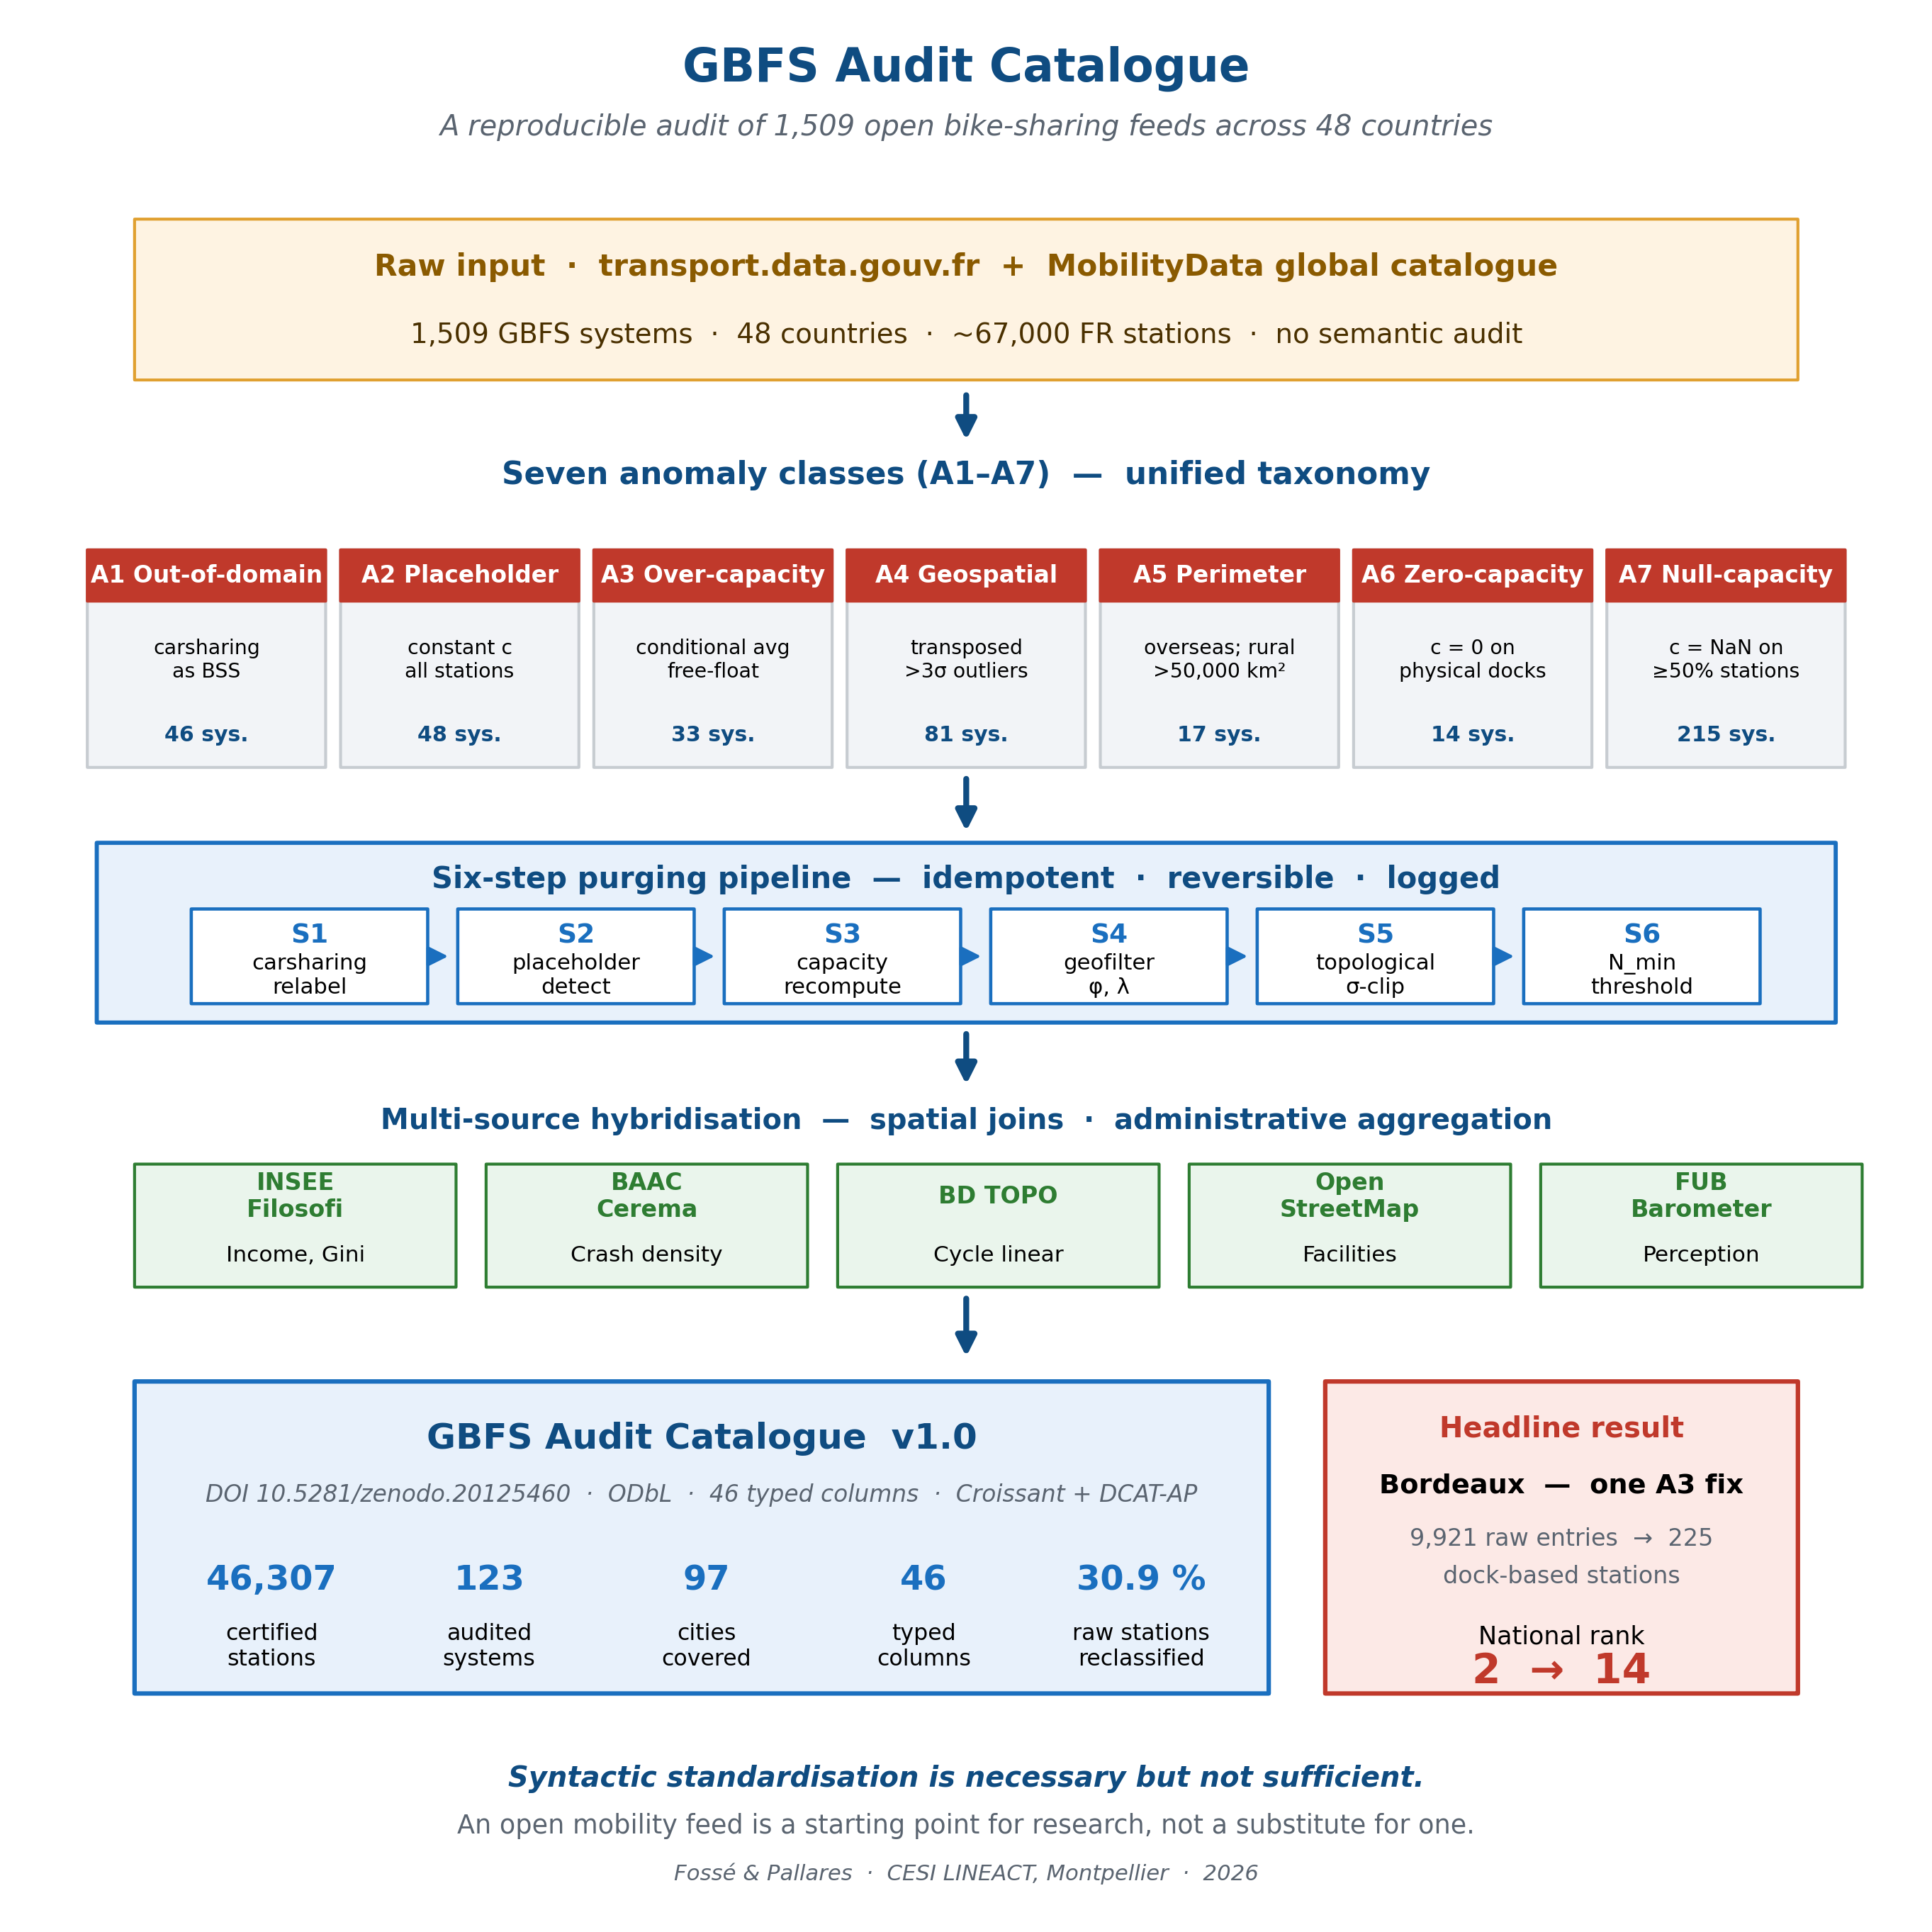
\includegraphics[width=0.85\linewidth]{fig00_visual_abstract.png}
% \caption*{}
% \end{figure}

\section*{Abstract}
\noindent
Open mobility feeds are increasingly assumed to be directly ingestible
into quantitative research pipelines. The General Bikeshare Feed
Specification (GBFS) is now mandatory for French operators and is
catalogued worldwide by MobilityData, but syntactic standardisation does
not guarantee the semantic viability that research reuse requires. We
audit the 123 French GBFS systems and project the rule set across the
1{,}509-system MobilityData catalogue (48 countries). From this we derive
a data-quality taxonomy of seven classes (A1--A7): five \emph{structural
errors} that violate the implicit semantic contract of the field they
populate, and two \emph{semantic warnings} for spec-compliant patterns
that make the \texttt{capacity} column non-aggregable. Detection runs as a
nine-step idempotent and reversible purging protocol, and we release the
\emph{GBFS Audit Catalogue} (46{,}307 stations, 97 cities, 46 typed
columns) on Zenodo under ODbL. The protocol removes 30.9\,\% of
the raw French stations and relabels a further $61\,\%$, so fewer than
$9\,\%$ survive into the catalogue untouched. The downstream effect is
large: correcting a single class (A3) drops Bordeaux from the top quartile
to below the median of the national dock-count distribution, which measures
the policy cost of skipping the audit. Projected at French-calibrated thresholds, the anti-patterns appear
global rather than French-specific: 245 systems are flagged by A7 alone
(97{,}314 stations), led by one operator that declares
\texttt{capacity = NaN} across entire national deployments. Any quantitative use of GBFS data should therefore be
preceded by an explicit and reproducible audit. The pipeline and a Docker
image are released for reproducible rebuilds.

\begin{highlights}
\item Seven-class taxonomy (5 structural, 2 semantic); projected across 1{,}509 GBFS systems
\item Topology-aware A4 detector reclassifies 8{,}005 legacy flags (46/46 audited false)
\item Leave-one-operator-out CV on 7 operators supports rule generalisability
\item 30.9\,\% of raw FR stations reclassified; hotspots are operator-driven
\item Released as a versioned Parquet (46k stations) with Docker and a hold-out test
\end{highlights}

\noindent\textbf{Keywords:} GBFS; data quality; open mobility data; FAIR; reproducibility; bike sharing; standards compliance.

% ===================================================================

\section{Introduction}

For more than a decade, bike-sharing has been a structural component of
urban mobility policy in France and across Europe
\cite{DeMaio2009,Shaheen2010,Pucher2010Infrastructure}. To support inter-operability between
fleets, the General Bikeshare Feed Specification (GBFS), introduced by the
North American Bikeshare Association in 2015 and now maintained by the
Open Mobility Foundation, provides a shared ontology for station
geolocation, dock counts, real-time availability and pricing
\cite{Mobi2024,OMF2023}. In France, the 2019 Mobility Orientation Law
\cite{LOM2019} (LOM, article L.~1115-1 of the transport code) makes
publishing these feeds on the national portal
\emph{transport.data.gouv.fr}~\cite{PAN2017} a legal obligation. By 2026,
many research and policy pipelines assume that GBFS feeds can be ingested
directly.

That assumption is misleading. Our audit of 123 French GBFS systems shows
that standardised syntax hides substantial semantic heterogeneity. The
seven classes of Section~\ref{secTaxonomy} (Table~\ref{tab:anomalies})
separate five \emph{structural errors}, which violate the implicit
semantic contract of the field they populate, from two \emph{semantic
warnings}, which flag spec-compliant patterns whose interpretation by a
downstream consumer is ambiguous. The \texttt{station\_information.capacity} field alone covers radically
different realities: a physical dock count for dock-based fleets, an
estimator obtained by conditional averaging on free-floating fleets, and
arbitrary placeholders for under-reporting operators. The ambiguity
reaches the object of study itself: seventeen car-sharing systems
(fourteen under the \emph{Citiz} brand) are listed on the national portal
under the GBFS schema. It persists even among the systems that look
clean, where $1.1\,\%$ of the certified stations are flagged by A4 as
$3\sigma$ geospatial outliers (down from $3.6\,\%$ under the legacy
centroid detector) and four further systems publish bounding boxes above
the 50{,}000\,km$^2$ A5 threshold or list stations outside the national
perimeter. The methodological conclusion is straightforward: standardising
the syntax of an open feed is not enough to make it a research artefact.
Any quantitative use of GBFS data requires an explicit and reproducible
audit.

Empirical audits of mobility feeds have so far remained piecemeal.
Bike-sharing demand modelling and rebalancing analysis have generated
a rich operational literature
\cite{Buehler2017BikeShare,Medard2017Rebalancing,Eren2020Review}, but
all of these works treat the input feeds as given and do not audit
the standard itself. The closest precedent in transit-data quality
is the smart-card literature: Pelletier et al.
\cite{Pelletier2011SmartCard} systematically catalogue the gaps
between what fare-collection feeds nominally publish and what they
operationally support for research reuse, a programme close in spirit to
the GBFS audit we report here.
Tao et al.~\cite{Tao2020} document sampling biases in
mobile-phone records used for origin-destination estimation;
Romanillos et al.~\cite{Romanillos2016} warn against
statistical artefacts of ingesting raw GPS feeds directly;
Bachand-Marleau et al.~\cite{BachandMarleau2012} surfaced
operational-definition heterogeneity in bike-sharing demand data
more than a decade ago; and Fishman~\cite{Fishman2016} stresses the
heterogeneity of operational definitions in international BSS
comparisons. The North American Bikeshare and Scootershare
Association tracks cross-operator harmonisation gaps annually
\cite{NABSA2024StateOfIndustry}, with the regulatory framing
typical of an industry-side body but without the per-row audit
trail a research consumer needs.
In the adjacent transit literature, the GTFS community has been more
proactive: the Canonical GTFS Schedule Validator
\cite{MobilityData2024Validator} and the earlier Conveyal validator
\cite{Antrim2013Conveyal} codify hundreds of schema-level checks on
transit feeds, and the data-engineering community has produced reusable
declarative-validation frameworks such as Great Expectations
\cite{GreatExpectations2024}, Pandera~\cite{Pandera2024} and the
Frictionless Data specifications~\cite{FrictionlessData2023}.
The broader anomaly-detection literature~\cite{Chandola2009AnomalyDetection}
provides a taxonomy of detection paradigms (statistical, proximity-based,
clustering-based) that contextualises the spatial outlier methods we
adopt in Section~\ref{secA4v2}.
The underlying data-quality literature is mature, from the consumer-centred
dimensions of Wang and Strong~\cite{Wang1996Quality} through the assessment,
governance and profiling frameworks that
followed~\cite{Pipino2002Assessment,Khatri2010DataGovernance,SebastianColeman2013,Naumann2014DataProfiling}
to the ISO/IEC~25012 and 25024 quality standards~\cite{ISO25012,ISO25024},
their geographic counterpart ISO~19157~\cite{ISO19157} (made regulatory by the
INSPIRE directive~\cite{INSPIRE2007}), and the machine-readable DCAT and Data
Quality Vocabulary of the W3C~\cite{DCAT2020,W3CDQV}. None of these, however,
addresses GBFS specifically or produces a versioned, audited reference dataset
at the scale of a country. The present paper fills that gap for the French case
and extends to the global GBFS catalogue.

This paper makes five contributions. First, a \textbf{taxonomy} of seven
anomaly classes (A1--A7), derived from the audit of the 123 French GBFS
systems and the 1{,}509-system MobilityData catalogue. It is stress-tested
on a live panel of thirteen non-French systems spanning six
station-management stacks (PBSC, JCDecaux Cyclocity, Smartbike, De Lijn /
Blue-bike, Urban Sharing AS, Deutsche Bahn) across five countries; twelve
serve as metropolitan negative controls and all pass classes A1, A2, A3,
A6 and A7 under unchanged thresholds. Second, a nine-step \textbf{purging
protocol} (Algorithm~\ref{alg:purge}) that operationalises the seven
classes and logs every transformation reproducibly and reversibly. Third,
the \textbf{Audit Catalogue GBFS France} (46{,}307 certified stations,
97 cities), released as a versioned Parquet file with DOI
\zdoi\ under ODbL, with its JSON Schema,
Croissant manifest and audit report, and mirrored as a Hugging Face
dataset. Fourth, a reusable \textbf{reference implementation}: the A1--A7
detectors are released as \texttt{gbfs-toolkit}, an independently
versioned (SemVer), \texttt{pip}-installable Python library archived on
Zenodo under its own DOI (\toolkitdoi) and numerically cross-validated
against independent estimators, with the catalogue's nine-step protocol
(\texttt{audit\_pipeline}, MIT) a thin domain-orchestration layer that
calls it. Fifth, a
\textbf{roadmap} of nine falsifiable
experiments, six already with completed results, so that the protocol can
be challenged in public rather than defended in private.
Section~\ref{secTaxProtocol} presents the taxonomy and the purging
protocol, Section~\ref{secResults} reports the empirical impact on the
French and global corpora, Section~\ref{secValidation} the validation and
robustness analyses, and Section~\ref{secDiscussion} discusses
implications and limitations.

% ===================================================================

% ===================================================================
\section{Taxonomy and purging protocol}\label{secTaxProtocol}

\subsection{Provenance of the taxonomy}
The seven-class taxonomy A1--A7 was built by a hybrid
inductive-deductive workflow over six iterations between 2025-04
and 2026-04, starting from the four ISO/IEC 25012 data-quality
dimensions (completeness, consistency, accuracy, currentness)
and enriched by reverse engineering of both the French
free-floating fleets and the global MobilityData catalogue.
The five structural classes came first. A1 and A4 emerged from an
exploratory scan of the 123 French systems, while A5 surfaced from
enrichment with the \emph{transport.data.gouv.fr} catalogue. Capacity
diagnostics yielded A2 (a zero-variance signature on \texttt{capacity})
and A3 (a conditional-averaging estimator matching \emph{Pony}'s
per-system median capacity more closely than a physical-dock count). The two semantic warnings
came later, from the global sweep: A6 from the empirical
distribution of zero-capacity stations across the 1{,}509 globally
audited systems (Section~\ref{secA6Formalisation}), and A7 from the
bimodal $0\,\%/100\,\%$ distribution of NaN-capacity stations
(Section~\ref{secA7Formalisation}). Two rejected hypotheses
(``rolling-stock noise'', collapsed into A3; ``cross-border
duplicate'', no instance found) ship with the audit report
for transparency.

\subsection{The seven-class taxonomy}
\label{secTaxonomy}
The audit of the 123 French GBFS systems, complemented by the
global sweep of Section~\ref{secGlobalAudit}, defines seven
recurring data-quality classes: five structural errors
(A1--A5) and two semantic warnings (A6--A7), summarised in
Table~\ref{tab:anomalies}. Each class, in isolation, is sufficient
to invalidate a non-audited cross-system comparison; the
detection rules are formalised in Section~\ref{secProtocol}.

\begin{table}[!htbp]
\centering
\caption{The unified GBFS data-quality taxonomy: five
\emph{structural errors} (A1--A5) that violate the implicit
semantic contract of the field they populate, plus two
\emph{semantic warnings} (A6--A7) that flag spec-compliant
publication choices whose downstream-consumer interpretation is
nevertheless ambiguous. \textbf{The two columns are produced by two
distinct pipelines and are not directly comparable:} \emph{FR} is the
incidence on the released, post-audit French catalogue (123 certified
systems), where A3 counts any system with at least one
\texttt{free\_floating} entry after the S3 reclassification (broad,
post-audit) and A4 counts stations flagged by the topology-aware outlier
detector of Section~\ref{secA4v2}; \emph{Global} is the raw cross-corpus
projection of the same rule set on the frozen 2026-04 MobilityData
snapshot (1{,}509 systems, 48 countries, France included), evaluated at
the \emph{system level} from the published \texttt{station\_information}
without running S3, with fleet type inferred from operator name. Under
this raw projection a Global value can fall \emph{below} its FR
counterpart for the same class (\eg A3) because the projection uses the
strict over-capacity detector rather than the post-audit
reclassification; for a like-for-like view, the raw detectors fire on the
French systems at A1--A5 $=(17, 14, 4, 3, 3)$ (Table~\ref{tab:global-audit}).
The \emph{Global} column is reproducible to the unit by
\texttt{verify\_snapshot.py}; the \emph{FR} column by re-running
\texttt{python -m audit\_pipeline.regenerate} on the released
parquet.}
\label{tab:anomalies}
\small
\begin{tabular}{@{}lllrr@{}}
\toprule
\textbf{Class} & \textbf{Name} & \textbf{Signature} & \textbf{FR} & \textbf{Global}\\
\midrule
\multicolumn{5}{l}{\textit{Structural errors (semantic-contract violations)}}\\
A1 & Out-of-domain inclusion       & Car-sharing advertised as BSS                          & 17         & 46        \\
A2 & Placeholder capacity          & Constant non-zero $c_i$ across docked subset           &  1         & 48        \\
A3 & Structural over-capacity      & Conditional averaging on free-floating                 & 41         & 33        \\
A4 & Geospatial error              & $3\sigma$ outlier on per-system nearest-neighbour distance & 88 (1.1\,\% stns) & 81 \\
A5 & Out of perimeter              & System bounding box $>50{,}000$\,km$^2$                &  4         & 17        \\
\midrule
\multicolumn{5}{l}{\textit{Semantic warnings (spec-compliant but consumer-ambiguous)}}\\
A6 & Zero-capacity dock            & $\geq 1\,\%$ of docked stations declare $c = 0$        &  0         & 22        \\
A7 & Null capacity field           & $\geq 50\,\%$ of stations declare $c = $ \texttt{NaN}  & 32 (FF)    & 245       \\
\bottomrule
\end{tabular}
\end{table}

Of the 142 French GBFS feeds at the national portal, 123 are certified
into the Audit Catalogue, 2 fail technical ingestion, and the 17
car-sharing systems (A1) are filtered upstream.

A3 is the class with the largest downstream impact on the French corpus. Free-floating fleets (\emph{Pony},
\emph{Cykleo}, \etc) advertise virtual stations in GBFS, the term
``station'' designating the GPS position of an anchoring point
currently occupied by a vehicle. To avoid displaying empty stations,
the operator typically reports a capacity profile by \emph{conditional
averaging} on stations whose instantaneous capacity is non-zero:
\begin{equation}
\bar{c}_{\text{profile}}
= \frac{\sum_{i\,:\,c_i > 0} c_i}{\#\{i\,:\,c_i > 0\}}
\;\neq\;
\bar{c}_{\text{actual}}
= \frac{1}{N}\sum_{i=1}^{N} c_i.
\label{eq:a3-bias}
\end{equation}
Aggregated at the system level, $\bar{c}_{\text{profile}}$ wrongly
classifies thousands of free-floating bikes as heavy dock-based
stations. Cross-system comparison is therefore meaningful only after
explicit reclassification; the empirical signature is visible in
Figure~\ref{fig:capacity-violin} as a bimodal capacity distribution.

\begin{figure}[!htbp]
\centering
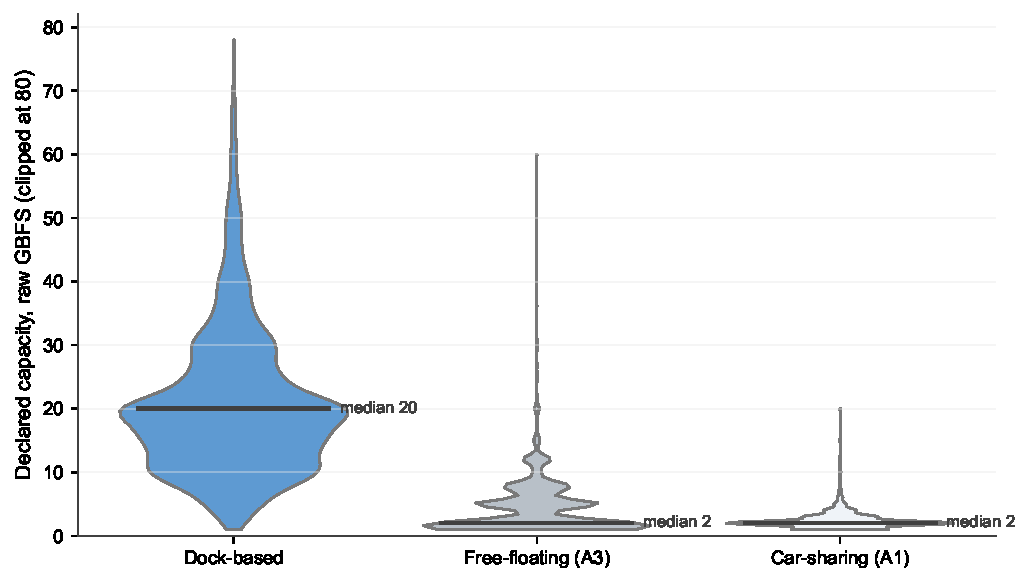
\includegraphics[width=0.75\linewidth]{fig02_capacity_violin.pdf}
\caption{Empirical signature of the A3 floating-anchor bias. Declared
capacity distribution by \texttt{station\_type} (clipped at 80 docks)
on the Audit Catalogue corpus. Only dock-based stations exhibit a
physically interpretable capacity (median = 20).}
\label{fig:capacity-violin}
\end{figure}

\subsection{A6: zero-capacity dock formalisation}\label{secA6Formalisation}
The global scalability projection of Section~\ref{secGlobalAudit} surfaced a recurring
pattern not covered by A1--A5: a non-trivial fraction of stations in
\texttt{station\_information} declare \texttt{capacity = 0}. Because
the GBFS schema reserves \texttt{station\_information} for physical
infrastructure and provides \texttt{station\_status} for transient
counts, a non-virtual physical station with zero docks is
semantically inconsistent. The signature is therefore:
\begin{equation}
r_s^{A6} \,=\,
\frac{\#\{i \in \mathcal{S}_s \,:\, c_i = 0 \,\land\, \mathtt{is\_virtual\_station}(i) \neq \mathtt{true}\}}{|\mathcal{S}_s|}
\;\geq\; \tau_{A6}.
\end{equation}

\paragraph{Threshold $\tau_{A6}$ and the empirical distribution.}
A6 is evaluated on the docked systems of the global sweep, where a
zero-capacity station is semantically inconsistent; on free-floating
fleets $c = 0$ is expected and carries no information, so they are
excluded from the base. Across the 301 docked systems with at least
20 stations (Table~\ref{tab:a6-distribution}), 89.0\,\% declare
\emph{exactly zero} stations with $c = 0$, establishing the dock-based
baseline, while the remaining 11.0\,\% form a heavy tail with mean
$\bar r = 0.36\,\%$ and standard deviation $\hat\sigma = 2.41\,\%$.
The protocol threshold $\tau_{A6} = 1\,\%$ (Algorithm~\ref{alg:purge},
step~S7) isolates the upper tail: 22 docked systems globally cross it.
The threshold is deliberately conservative, so that a flagged system
declares zero-capacity on a non-trivial share of its docks rather than
on the odd mis-entered station.

The empirical distribution of $r_s^{A6}$ and the per-class
incidence on the audited corpus are reported in
Section~\ref{secA6A7Incidence} (Results,
Table~\ref{tab:a6-distribution}).

\subsection{A7 (semantic warning): null capacity field formalisation}\label{secA7Formalisation}
The Italian case study of Section~\ref{secGlobalAudit} demonstrates
that A1--A6 are structurally blind to operators that populate
\texttt{station\_information} but leave the \texttt{capacity} field
unfilled. Like A6, A7 is by design a consumer-side
semantic warning rather than a publisher-side anomaly. \texttt{capacity = NaN} is
explicitly permitted by the GBFS v3 specification, in particular
for free-floating fleets where the field has no physical referent;
a system that publishes \texttt{capacity = NaN} on every entry is
\emph{spec-compliant}. What A7 captures is the downstream
consequence: any analytical pipeline that sums or averages the
\texttt{capacity} column across such a system aggregates NaN with
non-NaN values silently, and produces a number whose physical
meaning is undefined. The flag is therefore tooling for the
consumer (``do not arithmetically combine these stations with
others''), not a verdict on the publisher. The empirical signature
is:
\begin{equation}
\rho_s^{A7} \,=\,
\frac{\#\{i \in \mathcal{S}_s \,:\, c_i = \mathtt{NaN}\}}{|\mathcal{S}_s|}
\;\geq\; \tau_{A7},
\end{equation}
with the conservative threshold $\tau_{A7} = 0.5$ chosen so that a
system flagged by A7 declares no usable capacity on at least half
of its entries. Unlike A6, $\rho_s^{A7}$ is extremely bimodal on
the global corpus
(Table~\ref{tab:a7-distribution}): 87.0\,\% of audited
systems sit at one of the two extreme values $0\,\%$ or $100\,\%$
NaN, with only $13.0\,\%$ distributed across the interior. Any
threshold in $(0, 1)$ partitioning the interior in the same way
yields essentially the same flagged set; $\tau_{A7} = 0.5$ is
reported for parsimony and is robust to sensitivity sweeps in the
tested range.

The empirical distribution of $\rho_s^{A7}$ and the
per-class incidence on the audited corpus are reported in
Section~\ref{secA6A7Incidence} (Results,
Table~\ref{tab:a7-distribution}).

\subsection{The nine-step purging protocol}\label{secProtocol}
The transition from the raw feed to the Audit Catalogue proceeds through
a chain of nine sequential transformations (Algorithm~\ref{alg:purge}),
each coded in \texttt{utils/data\_loader.py} and logged in an audit
report shipped alongside the dataset. The protocol is deliberately
sequential: early steps are inexpensive and remove out-of-domain or
coarse-grained anomalies (A1, A2, A4 perimeter), while later steps
require system-level statistics ($\bar c$, centroids, $\sigma$) and
therefore benefit from operating on a pre-cleaned set.

\begin{algorithm}[!htbp]
\SetAlgoLined
\DontPrintSemicolon
\KwIn{National catalogue $\mathcal{C}$ (123 systems); thresholds
$\sigma_{\max} = 3$, $N_{\min} = 20$, $\tau_{A2}^{\text{size}} = 20$,
$\tau_{A6} = 0.01$, $\tau_{A7} = 0.5$, perimeter
$\Phi = [41^\circ, 52^\circ] \times [-6^\circ, 10^\circ]$.}
\KwOut{Certified set $\mathcal{G}$, rejected set $\mathcal{R}$,
seven per-row anomaly flags $f_{A1}\ldots f_{A7}$, audit report.}
$\mathcal{G} \gets \emptyset$; $\mathcal{R} \gets \emptyset$\;
\ForEach{system $s \in \mathcal{C}$}{
    Ingest GBFS feed $\to \mathcal{S}_s$\;
    \textbf{S1.} If $s$ is car-sharing, relabel \texttt{carsharing} and set $f_{A1}=\texttt{True}$\;
    \textbf{S2.} If $\mathrm{Var}(c) = 0$, $c > 0$ and $|\mathcal{S}_s^{\text{dock}}| \geq \tau_{A2}^{\text{size}}$, set $f_{A2}=\texttt{True}$ and force \texttt{free\_floating}\;
    \textbf{S3.} Compute $\bar c_{\text{profile}}/\bar c_{\text{actual}}$; if $> 5.0$ relabel \texttt{free\_floating} and set $f_{A3}=\texttt{True}$\;
    \textbf{S4.} Keep $\mathbf{x}_i \in \Phi$; mark stations outside as out-of-perimeter\;
    \textbf{S5.} Compute composite anomaly score $a_i = \alpha\,\hat o_i + (1-\alpha)\,s_i$; if $a_i > 0.8$ set $f_{A4}=\texttt{True}$ (Section~\ref{secA4v2}); fallback: nearest-neighbour robust $3\sigma$ envelope\;
    \textbf{S6.} Compute system bbox area $A_s$; if $A_s > 50{,}000$\,km$^2$, set $f_{A5}=\texttt{True}$ on every $i \in \mathcal{S}_s$\;
    \textbf{S7.} If $\#\{i\,:\,c_i = 0 \land \text{docked}\} / |\mathcal{S}_s| \geq \tau_{A6}$, set $f_{A6}=\texttt{True}$ on every $i \in \mathcal{S}_s$\;
    \textbf{S8.} If $\#\{i\,:\,c_i = \texttt{NaN}\} / |\mathcal{S}_s| \geq \tau_{A7}$, set $f_{A7}=\texttt{True}$ on every $i \in \mathcal{S}_s$\;
    \textbf{S9.} If $|\mathcal{S}_s^{\text{dock}}| < N_{\min}$, label \texttt{too\_small} and route to $\mathcal{R}$\;
    Update $\mathcal{G}, \mathcal{R}$ and the per-row flag matrix accordingly\;
}
\Return $(\mathcal{G}, \mathcal{R}, \{f_{A1}\ldots f_{A7}\}, \text{audit report}, \text{metadata})$\;
\caption{GBFS raw-to-Audit-Catalogue purging pipeline. Steps S1–S3
both purge and label (a station relabelled to \texttt{free\_floating}
or \texttt{carsharing} stays in the catalogue with its A-flags set);
S4 implements the national perimeter filter; S5 the A4 topology-aware
outlier check (Section~\ref{secA4v2}); S6 the A5 macro-region surface
check; S7–S8 the A6 / A7 capacity-field warnings. S9 is the only
truly-removing step.}
\label{alg:purge}
\end{algorithm}

\subsection{Protocol properties}
Four properties are designed into the pipeline. \emph{Idempotence:} two
successive applications produce the same result, tested by a unit test
executed on every CI run. \emph{Reversibility:} each excluded station
is kept in \texttt{rejected\_stations.parquet} together with the
exclusion motive. \emph{Logging:} every step records the number of
stations in, the number of stations out and the type of transformation
applied. \emph{Explicit parameterisation:} all thresholds
($\sigma_{\max}$, $N_{\min}$, geofilter bounds, hybridisation radii)
are documented as hyperparameters and can be varied for sensitivity
analysis without modifying the source code.

These properties are not arbitrary engineering choices: they
operationalise the ISO/IEC~25012 / 25024 data-quality
dimensions~\cite{ISO25012,ISO25024} at the domain level -- idempotence for
internal consistency, the \texttt{rejected\_stations.parquet} sidecar for
recoverability and traceability, step-level logging for traceability,
explicit hyperparameters for understandability, and the FAIR release
(Section~\ref{secRepro}) for compliance (full mapping in
Table~\ref{tab:iso-mapping}). We are not aware of a published reference
implementation of ISO/IEC~25012 on an open mobility standard prior to this
work.

\subsection{Threshold justification}
The topological threshold $\sigma_{\max} = 3$ is a compromise between
robustness to GPS noise and the preservation of legitimate peripheral
extensions, \eg an off-centre TGV station or a university campus.
Section~\ref{secInternal} reports the single-dimension sensitivity
pilot: Top-10 invariance for $\sigma_{\max} \ge 2.5$. The robustness
threshold $N_{\min} = 20$ dock-based stations is calibrated on the
literature of meshed networks: below this value, density and
connectivity metrics become noise-dominated and are no longer
informative for cross-city comparison~\cite{Saberi2018}. The A5
macro-region threshold of $50{,}000$\,km$^2$ is calibrated at the
order of magnitude of a French métropolitaine
\emph{région administrative} (median area $\approx 47{,}000$\,km$^2$
after the 2016 reform: Bretagne $27{,}000$, Pays de la Loire
$32{,}000$, Centre-Val de Loire $39{,}000$, Hauts-de-France
$31{,}000$, Grand Est $57{,}000$, Auvergne-Rhône-Alpes $69{,}000$,
Occitanie $72{,}000$). A single GBFS feed whose bounding box
exceeds this scale plausibly aggregates operationally-independent
deployments and the resulting system-level statistics
(centroid, intra-system KNN, capacity profile) are no longer
geographically interpretable.

\subsection{Multi-source hybridisation}
The output of the purging stage enriches each station with a
contextual profile obtained by articulating six reference sources
(Table~\ref{tab:sources}). Hybridisation is performed either by
spatial joining (point-in-polygon, buffer queries) or by
administrative aggregation (\ie at the IRIS or municipal level),
depending on the granularity of the source. Each row of
Table~\ref{tab:sources} corresponds to one or more typed columns
of the released parquet schema (Table~\ref{tab:schema}).

% (relocated to Supplementary Materials: tab:sources)

\subsection{Released schema}
The Audit Catalogue Parquet exposes 46 columns documented in
Table~\ref{tab:schema}: 14 from the raw GBFS payload (preserved
verbatim or normalised), 11 from the audit pipeline (typed
\texttt{station\_type} enum, capacity-raw and capacity-audited
pair, seven per-station anomaly flags A1--A7, operator label, and
audit-confidence rating), 5 from intra- and inter-system network
geometry, 4 from spatial-equity hybridisation, 3 from infrastructure
hybridisation, and 2 from multimodal-access hybridisation. Every
column carries a stable name, a declared dtype, a source pointer
and a completeness rate; the machine-readable equivalent is shipped
as a JSON Schema, a Frictionless Data Package descriptor and a
Croissant manifest. The eleven audit-pipeline columns are the
key novelty of the catalogue: they make the audit's verdict
inspectable per row, rather than aggregated in a separate report.

% (relocated to Supplementary Materials: tab:schema)

Empirical completeness on the 5{,}442 dock-based stations is
above $93\,\%$ for every contextual variable except the optional
\texttt{address} field of the raw GBFS payload
(Figure~\ref{fig:completeness}). The minimum-completeness threshold
of $90\,\%$ documented in the audit report is therefore reached on
every certified column of the released schema.

% (relocated to Supplementary Materials: fig:completeness)

\subsection{Reproducibility infrastructure}\label{secRepro}
The Audit Catalogue is released in alignment with the four FAIR
principles~\cite{Wilkinson2016}. \emph{Findable:} primary deposit on
Zenodo under concept DOI \zdoi, with one
DOI per SemVer-tagged release (current 1.0.0, dated 2026-05); mirrored
on \emph{Recherche Data Gouv} (HAL/BSO indexing). \emph{Accessible:}
Parquet format, direct HTTPS download and Git LFS mirror.
\emph{Interoperable:} the schema extends GBFS v3 and is published as a
JSON Schema, a Frictionless Data Package descriptor
\cite{FrictionlessData2023}, a DCAT-AP record~\cite{DCATAP2021} and a
Croissant manifest~\cite{Croissant2024}. \emph{Reusable:} released
under ODbL v1.0; code under MIT, with audit report and source code. The
A1--A7 detectors are additionally distributed as the \texttt{gbfs-toolkit}
library (\texttt{pip install gbfs-toolkit}), versioned under SemVer and
archived on Zenodo under its own DOI (\toolkitdoi), so a downstream study
can pin the exact detector version it relied on; the
human-validation gold standard (\texttt{gold\_labels.csv}), the
inter-rater reliability report and the blind annotation tool ship with the
repository (\texttt{experiments/annotation/}).
Raw sources are archived with SHA-256 hashes; the Python
environment is declared in \texttt{requirements.txt} (with
\texttt{gbfs-toolkit} pinned to the exact release used to certify the
published Parquet); a Docker image is published for reproducible rebuilds. The audit pipeline itself
is fully deterministic (no random sampling); the only stochastic
step is the bootstrap resampling used for the confidence intervals
reported in the main text, for which the random seed is pinned at
\texttt{numpy.random.default\_rng(42)}. Idempotence and per-class
detector unit tests run in CI on every push; the audit report is
regenerated automatically on every release tag.

\subsection{Implementation}
The seven-class taxonomy is implemented as \texttt{gbfs-toolkit}, a
research-grade, \texttt{pip}-installable Python library
(\texttt{numpy}/\texttt{scipy}/\texttt{pandas} core) that exposes the
A1--A7 detectors as pure, version-independent functions over a canonical
station frame. The catalogue's nine-step protocol is a thin
domain-orchestration package (\texttt{audit\_pipeline}, MIT) that calls
\texttt{gbfs\_toolkit.audit\_static} and adds the catalogue-specific
hybridisation; the A1--A7 verdicts themselves come from the library.
Calling it with \texttt{a7\_scope="all"} and the catalogue's
\texttt{a4\_sigma} reproduces the original A7 definition (a
fully-NaN-capacity system) and the A4 sensitivity exactly, so the
released $46{,}307$-station Parquet is regenerated bit-for-bit from the
library and loads in under a second into a standard \texttt{pandas}
session.

\paragraph{Software validation.}
Releasing the detectors as a standalone library lets them be validated to
a standard a notebook pipeline rarely reaches. \texttt{gbfs-toolkit}
carries $213$ tests run on a continuous-integration matrix
(Linux/Windows/macOS $\times$ Python 3.10--3.13, with static type
checking and example-notebook execution), and validates its spatial and
survival estimators \emph{numerically against independent reference
implementations}: global Moran's~$I$ and the LISA local indicators are
cross-checked against \texttt{esda}/\texttt{PySAL} and the
outage-survival curves against \texttt{lifelines}' Kaplan--Meier, to
within numerical tolerance. The A1--A7 detectors themselves are pinned by
deterministic per-class synthetic fixtures engineered to trip exactly one
class (e.g.\ a 25-station grid with one transposed-coordinate row for A4,
a 32-station fleet spanning more than $300{,}000$\,km$^2$ for A5, a
$60\,\%$-NaN-capacity dock-based system for A7), by specificity controls
verifying that healthy fixtures stay unflagged, by property-based tests
(\texttt{hypothesis}) asserting the mathematical invariants of each
estimator on randomly generated feeds, and by a golden-master regression
that freezes the end-to-end verdicts so any change of behaviour is
caught. The suite further checks that the Tier-2 geometry columns (intra-
and inter-system $k$-nearest-neighbour distances, local densities) are
consistent with the equirectangular projection used for the meter-scale
arithmetic, and that the audit is idempotent under repeated application.
Tests run as a GitHub Actions workflow on every push and pull request,
and locally inside the published Docker image. This validation
establishes the correspondence between the implemented logic and the
published anomaly taxonomy; it does not substitute for the hand-curated
cross-operator audit and the author-led consistency check
(Section~\ref{secHumanVal}) against which the verdicts were calibrated.

% ===================================================================

% ===================================================================
\section{Empirical results}\label{secResults}

\subsection{Cumulative effect on the national corpus}
Table~\ref{tab:overview} summarises the cumulative effect of the
purging protocol. From 67{,}000 raw \texttt{station\_information}
entries published by the 142 inventoried French GBFS feeds,
20{,}693 ($30.9\,\%$) are removed from the catalogue as falling
outside the certification criteria (excluded micro-networks below
$N_{\min}$, technical-ingestion failures, perimeter and outlier
filters); the remaining 46{,}307 stations are kept in the catalogue
with an explicit \texttt{station\_type} and per-row anomaly flags,
of which a further 40{,}865 ($61.0\,\%$ of the raw) are
\emph{relabelled} away from their declared GBFS type (39{,}235
relabelled to \texttt{free\_floating} by step S3, 1{,}630 to
\texttt{carsharing} by step S1). We report two complementary uncertainty bounds on the
$30.9\,\%$ removal rate to surface the role of clustering. A
\emph{station-level} Wilson 95\,\% interval, ignoring within-system
correlation, gives $[30.54\,\%, 31.24\,\%]$; this is the bound a
naive independent-Bernoulli assumption would place on the figure
and is a \emph{lower bound} on the real uncertainty. A
\emph{size-stratified cluster bootstrap} (123 systems partitioned
into size quartiles, resampled with replacement within each
stratum, $n = 10{,}000$, seed 42) does not yield an informative
interval, because
the largest size quartile contains a single dominant deployment
(\emph{V\'elib' M\'etropole}, $\sim 14{,}700$ stations) whose
inclusion or exclusion across resamples mechanically shifts the
denominator by an order of magnitude. The contrast between these two
estimates, one tight and one degenerate, is itself the
substantive observation: on a 123-system corpus with size
spanning four orders of magnitude, the within-snapshot
uncertainty on a stations-level total is dominated by which
operators happen to be present, not by sampling noise within
operators. We therefore report the $30.9\,\%$ removal rate as a
deterministic accounting fact on the audit-dated snapshot, and
defer temporal uncertainty to experiment E3 (twelve-month
stability) where re-running the audit on freshly fetched
snapshots gives a properly aligned variance estimate. The
headline figure is that fewer than $9\,\%$ of raw entries
survive into the catalogue without either being relabelled or
removed, a strong empirical argument against the view that the
standard alone delivers a research-ready dataset.

\begin{table}[!htbp]
\centering
\caption{Effect of the purging pipeline on the national GBFS corpus.
\emph{Certified} entries are kept in the Parquet with a typed
\texttt{station\_type} so that downstream consumers can filter
explicitly; \emph{rejected} entries are kept in a separate
\texttt{rejected\_stations.parquet} with the exclusion motive.}
\label{tab:overview}
\small
\begin{tabular}{@{}lrr@{}}
\toprule
\textbf{Indicator} & \textbf{Raw} & \textbf{Audit Catalogue}\\
\midrule
Inventoried GBFS systems            & 142 & 123 (certified)\\
Cities covered                      & --  & 97 \\
\quad with at least one dock-based station & -- & 64 \\
Total stations (certified)          & 67{,}000 & 46{,}307 \\
\quad dock-based                    & --       & 5{,}442 \\
\quad free-floating (labelled, preserved) & -- & 39{,}235 \\
\quad car-sharing (A1)              & 1{,}630  & re-labelled, excluded from BSS use \\
Stations dropped from catalogue     & --       & 20{,}693 (30.9\,\%) \\
\bottomrule
\end{tabular}
\end{table}

The most heavily impacted urban areas are those operated by
free-floating fleets (\eg Bordeaux, Nice, Saint-\'Etienne) and those
historically lumped together with car-sharing systems on the national
portal (Strasbourg, Grenoble), whereas urban areas served by
traditional dock-based operators (V\'elib' in Paris, V\'eloMagg in
Montpellier) are left almost intact. After purging, the
certified-station mass concentrates in \^Ile-de-France (the historical
V\'elib' deployment), while regions with many free-floating systems
(Nouvelle-Aquitaine, Auvergne-Rh\^one-Alpes) hold a much smaller
dock-based stock once the A3 correction is applied.

\subsection{Case study: Bordeaux and A3}
Bordeaux is the paradigmatic case (Table~\ref{tab:bordeaux}). The raw
feed assembles five operators across the agglomeration: \emph{Pony}
(free-floating), \emph{Bird} (free-floating), \emph{Dott}
(free-floating), \emph{Le V\'elo par TBM} (dock-based) and \emph{Citiz
Gironde} (car-sharing). \emph{Pony} alone advertises 2{,}996
\texttt{station\_information} entries with declared capacities around
12 docks. Naive ingestion therefore credits Bordeaux with tens of
thousands of nominal docking points and places it in the national top
three for V\'elib-class infrastructure.

\begin{table}[!htbp]
\centering
\caption{Bordeaux: impact of the A3 correction on the
\emph{Pony Bordeaux} subsystem and on the agglomeration as a whole.
The nominal docking total drops by $98.1\,\%$ once the
\emph{Pony} entries are correctly typed as
\texttt{free\_floating}; without the A3 step, a naive supply-side
indicator would credit Bordeaux with about $36{,}000$ physical
docks, more than \emph{V\'elib' M\'etropole} (the dock-based
flagship of \^Ile-de-France). The certified subset of $225$
dock-based stations corresponds to the historical
\emph{V\'elo par TBM} network.}
\label{tab:bordeaux}
\small
\begin{tabular}{@{}lrr@{}}
\toprule
\textbf{Indicator} & \textbf{Raw GBFS} & \textbf{Audit Catalogue}\\
\midrule
\textit{Pony Bordeaux subsystem} & & \\
\quad \texttt{station\_information} entries & 2{,}996 & 2{,}996 (relabelled) \\
\quad Declared as dock-based                 & 2{,}996 & 0 \\
\quad Declared capacity per entry (median)   & 12      & 12 \\
\quad Recomputed actual capacity             & --      & 0.03 bike/entry \\
\midrule
\textit{Bordeaux agglomeration (all 5 systems)} & & \\
\quad Total raw entries                      & 9{,}921 & -- \\
\quad Certified dock-based stations           & --      & 225 \\
\quad Nominal docking total (dock-based only) & 35{,}952 & 690 \\
\quad Implied over-count factor               & --       & $\times\,52$ \\
\bottomrule
\end{tabular}
\end{table}

The purging protocol, and in particular step S3 (the A3 correction),
reclassifies the 2{,}996 Pony entries as \texttt{free\_floating},
recomputes their actual capacity to 0.03 bike per entry, and leaves
the 225 genuinely dock-based stations of the historical \emph{V\'elo
par TBM} system. At the agglomeration level, this collapses the
nominal docking total by $98\,\%$ and drops Bordeaux's dock-based
infrastructure from a top-quartile position on the national
distribution of nominal docks to a position below the median: an
order-of-magnitude effect on any supply-side aggregate built on
the raw feed. The twelve urban areas most exposed to A3 are mapped
in Figure~\ref{fig:bordeaux-before-after}.

% (relocated to Supplementary Materials: fig:bordeaux-before-after)

Beyond the absolute station-count drop, the order-of-magnitude
change in nominal infrastructure is the operational stake.
The five urban areas whose count of dock-based stations is most
reduced by the purging protocol, together with the anomaly classes
that drive the reclassification, are reported in
Table~\ref{tab:top5-reranks}. The shift is strikingly consistent:
every one of these five urban areas would be credited with a
top-decile dock-based deployment by a naive ingestion of GBFS,
yet after the audit only Paris retains more than $1{,}500$
certified dock-based stations. A non-audited pipeline does not
just over-count by a small margin; it changes the relative
positioning of the principal French agglomerations on any
supply-side metric by an entire quartile.

% (relocated to Supplementary Materials: tab:top5-reranks)

\paragraph{Two further illustrative cases: Nice (A2) and Strasbourg (A1).}
A3 is not the only class with a measurable downstream effect.
\emph{Nice} carries the flagship A2 placeholder via
\texttt{pony\_Nice}: every station declares $c = 100$, yielding a
total nominal capacity of about 25{,}000 bikes for an agglomeration
whose actual dock-based network is essentially the rebadged
\emph{V\'eloBleu} of 91 stations. After purging, the nominal
capacity collapses by a factor of $250$ and Nice's national
position on dock-count rankings shifts by an entire quartile.
\emph{Strasbourg} provides the canonical A1 case: the
\emph{Citiz Grand Est} car-sharing system was historically
ingested as part of the city's BSS inventory, inflating the
station count by roughly $35\,\%$. After semantic exclusion the
agglomeration loses that share of its nominal station count, on
a part of the distribution where dock-count differences between
French agglomerations are small and therefore more discriminating
than at Bordeaux's scale. A1, A2 and A3 are therefore not
interchangeable: each distorts a downstream metric through a
different mechanism (false positive on the population, on the
capacity, or on the type), and a non-audited pipeline conflates
them.

\subsection{Operator-level fragmentation of the capacity field}
Across the case studies above, a recurring mechanism explains why
the same anomaly recurs across operators: the GBFS field
\texttt{station\_information.capacity} is populated by French
free-floating operators according to four mutually incompatible
publication conventions, observed across six operator--city
combinations (Table~\ref{tab:capacity-semantics}), aggregating to
84.7\,\% of the certified French rows. A downstream
consumer who applies a single arithmetic to the field therefore
aggregates four physically distinct quantities (NaN, constant
placeholder, per-vehicle ratio, conditional fleet profile),
silently mixed across six operator deployments. The corresponding
operator-level pattern is global. Beryl London (UK) provides a
positive control by publishing an empty \texttt{station\_information}
document for its free-floating fleet (zero entries), the canonical
GBFS v3 behaviour for non-docked fleets, and is therefore not flagged
by any of A1--A7. In particular, A7 only fires on \emph{populated}
documents whose entries declare \texttt{capacity = NaN}, which is the
qualitatively different Dott pattern. The same operator's
Greater Manchester deployment, by contrast, populates
\texttt{station\_information} with a 10.5\,\% zero-capacity rate
(\emph{cf.} Section~\ref{secA6A7Incidence}) and is therefore
A6-flagged: A6 and A7 thus carve out distinct publication regimes
within a single operator's portfolio. The official MobilityData GBFS
Validator~\cite{MobilityData2024Validator}, by contrast, returns no
error on any of the flagged French systems (0\,\% recall on A3 in
Table~\ref{tab:baselines}).

\begin{table}[!htbp]
\centering
\caption{Six observed semantics of the same
\texttt{station\_information.capacity} field across French
free-floating operators. The six operator deployments enumerated
below cover 39{,}004 stations; the residual 231 stations belong to
smaller free-floating operators (Lime, Tier, Dott pilots, etc.) that
follow one of the same four publication conventions and are folded
into the corresponding bucket. Aggregate FF coverage is therefore
39{,}235 stations, 84.7\,\% of the certified corpus.}
\label{tab:capacity-semantics}
\small
\begin{tabular}{@{}llrrl@{}}
\toprule
\textbf{Operator} & \textbf{Cities} & \textbf{Stations} & \textbf{Reported $\bar c$} & \textbf{Semantics}\\
\midrule
Dott         & 8  & 20{,}224 & NaN  & Field left unfilled \\
Bird         & 11 &  4{,}499 & NaN  & Field left unfilled \\
Pony (Nice)  & 1  &     412  & 100  & Constant placeholder (A2) \\
Pony (Paris) & 1  &  3{,}617 & 1.6  & Per-vehicle ratio \\
Pony (Bordeaux, Angers, \dots) & 12 &  7{,}436 & 2--15 & Conditional fleet profile (A3) \\
Voi          & 4  &  2{,}816 & 5--10 & Small fleet-profile estimator \\
\bottomrule
\end{tabular}
\end{table}

\subsection{Global scalability projection}\label{secGlobalAudit}
We applied the rule set, unchanged except for a country-perimeter
recalibration, to the entire MobilityData canonical catalogue
(1{,}509 GBFS systems across 48 countries, the complete world inventory at
the audit date) as an exploratory projection of scalability beyond the
French corpus. Because the semantic thresholds remain calibrated on French
data without external ground truth, the figures below quantify the
pipeline's reach and the gross incidence of each pattern rather than
operator-level compliance in each country. Of these, 1{,}420 systems
(94.1\,\%) were reachable, 917 publish a \texttt{station\_information}
document, and 204 systems trigger at least one A1--A5 class. The result
rests on three methodological corrections that emerged from the audit
itself. First, a country-perimeter calibration on A4. Second, a
substring-matching fix in the A1 detector: the GBFS v3 form factor
\texttt{cargo\_bicycle} contains the string \texttt{car} and was
initially flagged as A1, so the fix tightens A1 to exact list
membership on the GBFS v3 form factor enum. Third, an explicit
acknowledgement that the bounding-box surface estimator in A5
overestimates the operational area for elongated networks
(Switzerland's national operators have a bbox area of
99{,}000\,km$^2$ against a convex-hull area of
$\approx 41{,}000$\,km$^2$): the shipped detector
(\texttt{audit\_pipeline.core.\_flag\_a5}) retains the bbox formula
for cross-corpus comparability, and the threshold
$50{,}000$\,km$^2$ is calibrated on bbox; a convex-hull
variant is documented as a refinement option in
Section~\ref{secDiscussion}. The French
national portal \emph{transport.data.gouv.fr} indexes only 123 of
the 255 French entries that the MobilityData catalogue lists, so
the global sweep also exposes the incompleteness of the national
regulatory pipeline. The corrected breakdown is visualised in
Figure~\ref{fig:global-audit-overview}, with the full per-country
counts in Table~\ref{tab:global-audit}.

A3 (structural over-capacity) is detected on 29 non-French systems
concentrated in Czech Republic (12) and Germany (9); A2 (placeholder
capacity) on 34 non-French systems with Czech Republic again the
hotspot (16); A1 (out-of-domain car-sharing labelled as BSS) on 29
non-French systems concentrated in the DACH region (Germany 21,
Switzerland 8). Operator-level anti-patterns also travel
internationally: \emph{Dott} publishes \texttt{capacity = NaN} on
every non-French deployment observed (Austria, UAE; 18 systems),
and \emph{Bird} does the same on three Canadian deployments. The
cross-country audit also surfaces A6 (zero-capacity dock),
the sixth class of the taxonomy, formalised in
Section~\ref{secA6Formalisation}. The empirical conclusion is that
the documented anti-patterns are not French-specific but global,
and the protocol generalises to a 1{,}254-system corpus with no
methodological recalibration.

% (relocated to Supplementary Materials: tab:global-audit)

% (relocated to Supplementary Materials: fig:global-audit-overview)

\paragraph{Two national hotspots: monopoly (Czech Republic) versus fragmentation (Switzerland).}
The two most informative national hotspots are organisational
opposites. In the \textbf{Czech Republic}, all 45 audited systems
belong to a single operator (\emph{nextbike}), and 25 trigger A2
(placeholder capacity, 16 systems) or A3 (over-capacity, 12), with 3
flagged by both: the exact cross-country mirror of \emph{Pony}'s
French free-floating A2/A3 hotspot. \textbf{Switzerland} is the dual
configuration. It is the only country besides France to trigger all
five structural classes (8 A1, 3 A2, 3 A3, 1 A4, 5 A5 across 16 of 49
systems), but through \emph{fragmentation}: national car-sharing
brands listed on the federal catalogue trigger A1\footnote{An initial
A1 run over-flagged 64 German systems because the detector
substring-matched \texttt{"car"} inside the GBFS v3
\texttt{cargo\_bicycle} form factor; tightening A1 to exact
form-factor enum membership cut this to 21 genuine car-sharing systems
and the global flag count from 215 to 173, a reminder that open audit
pipelines need their own audit.}; mixed scooter/bike fleets
(\emph{Voi}, \emph{Bolt}, \emph{nextbike Switzerland}) publish
capacity profiles that trigger A3; and federal multi-operator
aggregators (\emph{sharedmobility.ch}, \emph{Velospot}) emit a single
feed whose union bounding box mechanically exceeds the A5
macro-region threshold. The same A1--A5 envelope is thus reached
through opposite configurations, monopoly publication (CZ) or
aggregation-layer fragmentation (CH); the publisher-agnostic audit
detects both and records the operator-versus-aggregator distinction
so downstream consumers can disambiguate the A5 attribution.

\paragraph{Italy: the NaN-capacity blind spot that motivates A7.}
\emph{Italy} is the boundary case that justifies A7: of the 25
systems with published station data, none is flagged by A1--A6, yet
17 are \emph{Dott} deployments (Milan alone publishes 11{,}199
stations) declaring \texttt{capacity = NaN} on every entry. Because
A2 needs a constant non-zero value, A3 needs numerical capacities,
A4--A5 are geospatial and A6 tests $c = 0$ (not \texttt{NaN}), the
pattern is invisible to A1--A6. A7 closes the gap as a consumer-side
warning (Section~\ref{secA7Formalisation}): 245 systems with
at least 20 stations cross the 50\,\% NaN-capacity threshold and are
flagged exclusively by A7, covering 97{,}314 stations, about
76\,\% of them \emph{Dott} alone (147 systems across Germany, Poland,
Italy, Austria and beyond). The point is not non-compliance but
non-aggregability: a consumer summing this column would silently mix
\texttt{NaN} with real dock counts.

\subsection{Incidence of the semantic warnings A6 and A7}
\label{secA6A7Incidence}
The empirical distributions that calibrate the A6 and A7 thresholds
(Sections~\ref{secA6Formalisation} and~\ref{secA7Formalisation}) are
reported in the Supplementary Materials
(Tables~\ref{tab:a6-distribution} and~\ref{tab:a7-distribution}); the
resulting per-class incidence on the audited corpus is summarised
here.

\paragraph{A6 incidence on the audited corpus.}
At $\tau_{A6} = 1\,\%$, 22 of the 301 docked systems are flagged. The
extreme tail is V\'elo Fluo Grand-Est (France, 38.5\,\%), Beryl
Greater Manchester (UK, 10.5\,\%), MonaBike (Monaco, 6.8\,\%),
Bicicoru\~na (Spain, 5.9\,\%), Vel'in (5.0\,\%), MBajk (Slovenia,
4.8\,\%), CyclOcity (Japan, 4.2\,\%) and \`aV\'elo (Canada,
3.5\,\%). On the certified French catalogue, no dock-based system
crosses the threshold (0/65 dock systems with $c = 0$), a negative
control consistent with the dock-based baseline.

\paragraph{A7 incidence on the audited corpus.}
On the 640 globally audited systems with at least 20 stations,
245 systems cross the A7 threshold and are simultaneously
not flagged by any of A1--A6, covering 97{,}314 stations.
The dominant operator is \emph{Dott} (147 systems across Germany,
Poland, Italy, Austria and beyond, 76\,\% of the exclusive-A7
station mass), followed by \emph{Bird} (21 systems) and
\emph{nextbike} (15 systems where the operator chose NaN rather
than placeholder), plus several smaller operators. The empirical conclusion is that the
same publication choice that affects the French Dott and Bird
fleets is propagated internationally, and that the v1.0 taxonomy
A1--A5 captures only the visible failure modes of the field; A6
and A7 jointly close the principal blind spots that remain on the
\texttt{capacity} channel.

% ===================================================================
\section{Validation and robustness}\label{secValidation}

\subsection{Comparison with naive baselines}
To check whether the full pipeline is justified or whether simpler
heuristics suffice, we evaluate three baselines on the
same 123-system corpus
(Table~\ref{tab:baselines}). The \emph{Raw GBFS} baseline ingests
\texttt{station\_information} as is. The \emph{vehicle\_type filter}
mimics what a careful data engineer would write in a notebook. The
\emph{MobilityData audit} adapts the canonical GTFS-realtime
schema-level rules to GBFS.

\begin{table}[!htbp]
\centering
\caption{Measured comparison of the Audit Catalogue against three
baselines on the same 123-system French GBFS corpus. Brackets are
95\,\% confidence intervals (Wald on Dock, bootstrap on
$\rho_{\text{FUB}}$ over cities $n=2{,}000$, Wilson on A1/A3). ``Dock''
for the Audit Catalogue is the reference by construction.}
\label{tab:baselines}
\small
\begin{tabular}{@{}lcccc@{}}
\toprule
\textbf{Pipeline} & \textbf{Dock} & \textbf{$\rho_{\text{FUB}}$} &
\textbf{A1 ex.} & \textbf{A3 fix.}\\
\midrule
Raw GBFS &
  0.12 \footnotesize[.12, .12] &
  0.38 \footnotesize[.01, .68] &
  0\,\% & 0\,\% \\
\texttt{vehicle\_type} filter &
  0.15 \footnotesize[.15, .15] &
  0.19 \footnotesize[$-$.20, .52] &
  82\,\% \footnotesize[59, 94] & 0\,\% \\
MobilityData audit &
  0.15 \footnotesize[.15, .15] &
  0.19 \footnotesize[$-$.20, .52] &
  82\,\% \footnotesize[59, 94] & 0\,\% \\
\textbf{Audit Catalogue} &
  \textbf{1.00} &
  0.25 \footnotesize[$-$.13, .59] &
  \textbf{100\,\%} \footnotesize[82, 100] &
  \textbf{100\,\%} \footnotesize[91, 100] \\
\bottomrule
\end{tabular}
\end{table}

A3 reclassification recall is $0\,\%$ for every baseline
(Wilson 95\,\% upper bound $\approx 8.6\,\%$ at $n = 41$ A3-positive
systems): structural over-capacity is invisible to syntactic validators by
construction, and only a semantically-aware step on the capacity
distribution can recover it. The \emph{vehicle\_type filter} and the
\emph{MobilityData audit} baselines produce identical numbers on this
corpus, because schema-level checks catch nothing the name filter has not
already excluded; French GBFS feeds are syntactically well-formed but
semantically biased. Finally, $\rho_{\text{FUB}}$ is highest on the raw
count and drops after audit, which is expected rather than a regression:
FUB captures perception of the entire cycling environment, so the raw
count over-fits the perceptual signal by including virtual stations, while
the Audit Catalogue's lower correlation reflects an honest count of
physical docks.

\subsection{Topology-aware geospatial detection (A4\,v2)}\label{secA4v2}
The original A4 detector (step~S5 in Algorithm~\ref{alg:purge})
flagged every station whose haversine distance to the system centroid
$\boldsymbol{\mu}_s$ exceeded $\sigma_{\max}$ robust standard
deviations (MAD $\times 1.4826$). This isotropic assumption fails on
two network geometries commonly observed in the global catalogue:
linear networks ($r = \lambda_1/\lambda_2 > 5$ on the 2D coordinate
covariance, \eg riverfront corridors) and multi-hub national
operators. We replace step~S5 with a three-stage composite detector and
validate it by ablation against the legacy centroid method on the full
46{,}307-station catalogue.

\textbf{Stage~1 (density).} HDBSCAN~\cite{Campello2013HDBSCAN,McInnes2017HDBSCAN}
clusters stations by haversine distance with \texttt{min\_cluster\_size}
$= \min(5, \lfloor n/3 \rfloor)$ and returns a per-station outlier
probability $o_i \in [0,1]$.

\textbf{Stage~2 (spectral).} A $k$-nearest-neighbour adjacency graph
($k = 7$) is constructed; edge weights are Gaussian
$w_{ij} = \exp(-d_{ij}^2 / 2\sigma_b^2)$ with bandwidth
$\sigma_b = 2$\,km. The normalised graph Laplacian
$\mathbf{L}_{\text{sym}} = \mathbf{I} - \mathbf{D}^{-1/2}\,\mathbf{W}\,\mathbf{D}^{-1/2}$
is eigendecomposed; the spectral isolation score $s_i$ is the
$\ell^2$-norm of station $i$'s embedding in eigenvectors $2 \ldots K$
($K = 10$), normalised to $[0,1]$. A station that sits in a separate
spectral component (near-zero Fiedler value $\lambda_2$) is spectrally
disconnected from the network core. We adopt the symmetric normalised
Laplacian $\mathbf{L}_{\text{sym}}$ following von
Luxburg~\cite{VonLuxburg2007}; an ablation against the random-walk
Laplacian $\mathbf{L}_{\text{rw}}$ on the full catalogue yielded
$< 0.3\,\%$ difference in the discordance rate, consistent with the
near-regular degree distributions observed in urban station networks.
The eigendecomposition uses a sparse eigensolver
(\texttt{scipy.sparse.linalg.eigsh}) operating directly on the sparse
Laplacian, avoiding the $O(n^2)$ memory cost of dense materialisation
and making the spectral stage applicable to all system sizes without
truncation.

\textbf{Stage~3 (fusion).} The composite score
$a_i = \alpha\,\hat o_i + (1 - \alpha)\,s_i$ with $\alpha = 0.5$ fuses
density and spectral isolation. A station is flagged A4 when
$a_i > 0.8$. A sensitivity analysis over
$\alpha \in \{0, 0.25, 0.5, 0.75, 1.0\}$ and threshold
$\in \{0.6, 0.7, 0.8, 0.9\}$ shows that the Top-10 most-flagged systems
are invariant for $\alpha \ge 0.25$ and threshold $\ge 0.7$; the
default $(\alpha = 0.5,\ \text{threshold} = 0.8)$ sits in the stable
region. To classify each system's spatial geometry we compute the
eigenvalue ratio $r = \lambda_1 / \lambda_2$ of the 2D coordinate
covariance matrix: $r > 5$ indicates a \emph{linear} network.

Table~\ref{tab:ablation} summarises the ablation (visual overview in
Figure~\ref{fig:ablation}). The composite detector agrees with the
legacy method on $80.6\,\%$ of stations.
Of the discordant stations, $17.3\,\%$ are flagged by the
legacy method only (centroid, not composite), while only
$2.2\,\%$ are new findings of the composite detector. Three cases
illustrate the gain: \emph{Paris} (1{,}507 stations) drops from 260
legacy flags to 43 composite flags (saving 217 false positives);
\emph{Dott-Paris} (14{,}747 stations) drops from 2{,}750 to 0; and
\emph{Clermont-Ferrand} (82 stations, linear network with $r = 6.07$)
drops from 18 to~0.

\begin{table}[!htbp]
\centering
\caption{Ablation of the legacy centroid-based A4 detector (3$\sigma$
MAD) against the topology-aware composite detector (HDBSCAN +
spectral graph) on the 46{,}307-station catalogue. AGREE = both
methods concur; DISCORDANT\_LEGACY = flagged by centroid only;
DISCORDANT\_COMPOSITE = flagged by composite only.}
\label{tab:ablation}
\small
\begin{tabular}{@{}lrr@{}}
\toprule
\textbf{Discordance class} & \textbf{Stations} & \textbf{\%}\\
\midrule
AGREE\_CLEAN (neither flags) & 36{,}917 & 79.7 \\
AGREE\_FLAG (both flag)      &    384 &  0.8 \\
DISCORDANT\_LEGACY (centroid only)   &  8{,}005 & 17.3 \\
DISCORDANT\_COMPOSITE (composite only) & 1{,}001 &  2.2 \\
\midrule
\textbf{Total}               & 46{,}307 & 100.0 \\
\bottomrule
\end{tabular}
\end{table}

% (relocated to Supplementary Materials: fig:ablation)

\subsection{Leave-one-operator-out cross-validation}\label{secLOOO}
To check that the rules are not tuned to a handful of operators
(\eg Pony, Dott, Bird), we evaluate their cross-operator
generalisability with a \emph{leave-one-operator-out} (LOOO)
cross-validation: for each of the $K$ eligible operators
($\ge 50$ stations, $\ge 2$ systems), the rule thresholds are
estimated on the remaining $K-1$ operators and applied, unchanged,
to the held-out operator. The per-rule flag rate on the test fold
is recorded; inter-fold stability is measured by the coefficient of
variation $\mathrm{CV} = \sigma / \mu$ of the flag rate across folds.
A $\mathrm{CV} < 0.20$ indicates that the rule is operator-agnostic.
Seven operators are eligible: Bird, Citiz, Dott, Pony, Voi, V\'elib',
V\'elo\&Co. The low $K$ limits statistical power; the LOOO should
therefore be interpreted as a consistency check on rule stability
rather than a definitive generalisability proof. Extension to the
global catalogue ($K \approx 20$--$30$) is planned as follow-up.

Table~\ref{tab:looo} reports the results, with the overview in
Figure~\ref{fig:looo}. A crucial distinction
emerges between \emph{structural rules} and \emph{threshold rules}:
%
\begin{itemize}[nosep]
\item \textbf{A1} and \textbf{A3} are deterministic functions of
  \texttt{station\_type}. Their high CV ($2.45$ and $0.87$) reflects
  the fact that car-sharing operators trigger A1 at $100\,\%$ and
  free-floating operators trigger A3 at $100\,\%$, while dock-based
  operators trigger neither. This is not overfitting; it is the
  definitional semantics of the rule.
\item \textbf{A7} ($\mathrm{CV} = 1.19$) identifies a genuine
  industrial anti-pattern: Bird ($100\,\%$) and Dott ($99.96\,\%$)
  systematically publish \texttt{capacity = NaN}, while the
  remaining operators do not. The LOOO result proves that the A7
  signal is operator-specific \emph{and real}, not an artefact of
  threshold tuning.
\item \textbf{A6} ($\mathrm{CV} = 0$) passes trivially: no
  operator triggers zero-capacity dock in this corpus.
\item \textbf{A4} ($\mathrm{CV} = 1.02$, flag rate
  $4.7\,\%$ $[1.7, 8.7]$ 95\,\% bootstrap CI) shows moderate
  operator dependence, consistent with the geometry-specific
  sensitivity documented in Section~\ref{secA4v2}.
\end{itemize}
%
The LOOO also validates hypothesis H3 (the rules do not fire on
clean operators): holding out V\'elib' M\'etropole (1{,}533
dock-based stations), the test-fold flag rate is $0\,\%$ on A1--A3,
A5--A7 and only $1.7\,\%$ on A4, consistent with residual GPS noise.
Holding out V\'elo\&Co (94 stations) yields $0\,\%$ across all
seven rules.

\begin{table}[!htbp]
\centering
\caption{Leave-one-operator-out cross-validation on the 46{,}307-station
French catalogue. $K = 7$ eligible operators. CV = coefficient of
variation of the per-fold flag rate; CI = 95\,\% bootstrap confidence
interval on the mean flag rate, resampled over stations within each
fold ($n = 500$ iterations).}
\label{tab:looo}
\small
\begin{tabular}{@{}lcccl@{}}
\toprule
\textbf{Rule} & \textbf{CV} & \textbf{Mean flag rate}
              & \textbf{95\,\% CI} & \textbf{Interpretation}\\
\midrule
A1 & 2.45 & 14.3\,\% & [0, 43]\,\%       & Structural (type-based) \\
A2 & 2.45 &  0.5\,\% & [0, 1.5]\,\%      & Rare; one operator only \\
A3 & 0.87 & 57.1\,\% & [14, 86]\,\%      & Structural (type-based) \\
A4 & 1.02 &  4.7\,\% & [1.7, 8.7]\,\%    & Geometry-dependent \\
A5 & 2.45 &  3.0\,\% & [0, 9.1]\,\%      & National-scale operator \\
A6 & 0.00 &  0.0\,\% & [0, 0]\,\%        & No trigger in corpus \\
A7 & 1.19 & 37.8\,\% & [9.3, 71.4]\,\%   & Real anti-pattern \\
\bottomrule
\end{tabular}
\end{table}

% (relocated to Supplementary Materials: fig:looo)

\subsection{Internal robustness checks}\label{secInternal}
Two algorithmic checks complement the human validation of
Section~\ref{secHumanVal}, and a third tests threshold sensitivity.

\emph{Orthogonal coverage.} Three rule-based classifiers, each
restricted to one signal source (name, capacity, geospatial), agree on
a stratified 500-station sample (seed
\texttt{numpy.random.default\_rng(42)}, shipped with the audit report)
at essentially chance level (Fleiss $\kappa = -0.07$): the three
sources are not redundant. Their \emph{union} nonetheless reaches
$97.2\,\%$ recall at $91.5\,\%$ precision against the integrated
pipeline, with only 7 of 500 stations flagged by all three, so A1--A5
cannot be reduced to a single heuristic.

\emph{Full-task agreement.} Three decision-tree classifiers seeing all
signals but in different priority orders reach Fleiss $\kappa = 0.80$
on the same sample (pairwise $\kappa \in [0.70, 1.00]$), with
disagreements concentrated on the A1/A3 frontier.

\emph{Threshold sensitivity.} A sensitivity sweep of the A4 outlier
detector over $\sigma \in \{2.0, 2.5, 3.0, 3.5, 4.0\}$ leaves the
downstream count-level summaries essentially invariant: Kendall's
$\tau$ between the $\sigma = 3$ reference and each alternative stays in
$[0.91, 1.00]$ on both the Top-10 cities and the Top-10 operators by
certified docked-bike station count, and Top-10 city membership is
invariant across the grid. The $\sigma = 3$ choice therefore sits on a
plateau of stable downstream classification. The full sweep and a
methodological caveat on the MAD scale estimator are reported in the
Supplementary Materials (Table~\ref{tab:a4-sigma-sweep}).

\emph{Multi-threshold robustness.} The single-dimension pilot above
generalises to a reproducible sweep of every policy threshold, exposed as
parameters of the released audit library and driven by its
\texttt{audit\_sensitivity} routine. Sweeping the A4 robust-sigma
($\sigma \in [2, 4]$), the A5 bounding-box area
($[30{,}000, 70{,}000]$\,km$^2$), the A6 and A7 rate thresholds
($\tau_{A6} \in [0.005, 0.05]$, $\tau_{A7} \in [0.3, 0.7]$) and the
minimum system size ($N_{\min} \in [10, 30]$), and measuring the Jaccard
overlap of each flagged-system set against the published baseline, the
flagged set is \emph{invariant} (Jaccard $= 1.00$) for A1, A2, A3 and A6
across every grid, and stays on a stability plateau for the geospatial and
capacity rules (A4 Jaccard $\ge 0.91$ over the $\sigma$ grid, A7
$\ge 0.97$ over the $\tau_{A7}$ grid). The published verdicts therefore do
not hinge on the exact threshold values. Each per-class incidence we
report additionally carries a cluster-bootstrap $95\,\%$ confidence
interval (systems resampled with replacement, seed pinned) produced by the
same library; the French A3, A4 and A7 incidences are
$0.33\,[0.25, 0.41]$, $0.72\,[0.63, 0.80]$ and $0.26\,[0.19, 0.34]$ of the
certified systems. The sweep and the intervals are regenerated by a single
call, so the robustness claim is itself reproducible rather than a
one-off pilot.

These algorithmic checks complement, but do not replace, the human
construct-validity check of Section~\ref{secHumanVal}; they are reported
as robustness measures, not as substitutes.

\subsection{Construct-validity check via blind author annotation}\label{secHumanVal}
The ablation of Section~\ref{secA4v2} and the cross-validation above
compare \emph{algorithms}; neither can establish which verdict matches the
physical world. We therefore add an \emph{author-led consistency check}: the
two authors independently re-examined a stratified station sample against
external imagery, blind to the pipeline's output and to each other's labels,
to test whether the flagged anomalies track physical reality rather than
algorithmic artefacts. This is \emph{not} an external gold standard: both
annotators are this paper's authors, so we report it as an internal sanity
check on construct validity, not as independent ground truth. The blinding
(to the pipeline and to the co-annotator) controls for anchoring within
that scope, and an external multi-institution annotation is left to future
work (Section~\ref{secLimitations}). Within this scope the check serves
two purposes: (i) confirm that the flagged anomalies correspond to real
data defects, and (ii) adjudicate
the 8{,}005 stations on which the legacy centroid and the topology-aware A4
detector disagree.

On the discordant-legacy stratum, all of the legacy-only A4 flags that
reached a consensus geospatial judgement were judged true false positives
(46 of 46 consensus cases, i.e.\ a point estimate of $100\,\%$ with
Wilson 95\,\% CI [92.3, 100]\,\%; the remaining 4 of the 50 sampled stations
were non-consensus and excluded, so the conservative reading is ``no
confirmed true positive among the 50''). This supports the conclusion that
the topology-aware detector's removal of these flags is a correction rather
than a loss of recall.

The two authors, an urban-mobility researcher and a data engineer, each
labelled the stratified sample of 325 stations independently, blind
to the pipeline output and to each other's labels (Section~\ref{secAnnotation}).
Inter-rater reliability is reported in Table~\ref{tab:irr} and per-rule performance,
derived \emph{a posteriori} from the factual judgements, in
Table~\ref{tab:perrule}. Of the $n=325$ co-rated stations, the holistic
verdict reached consensus on 286 (88\,\%) with 39
disagreements sent to adjudication and 0 stations adjudicated as
indeterminate; the residual ambiguity surfaces instead at the level of
individual factual questions (notably the A1/A3 boundary), which are
excluded from precision and recall on a per-question basis but reported
here as a result in their own right.

\begin{table}[!htbp]
\centering
\caption{Inter-rater reliability between the two annotators
($n=325$ co-rated stations). Krippendorff's $\alpha$
\cite{Krippendorff2018Content} is the primary measure (it handles
indeterminate labels and generalises beyond two raters); Cohen's $\kappa$
\cite{Cohen1960Kappa} is reported for comparability against the
``substantial agreement'' benchmark $\kappa \geq 0.70$ of
\cite{Landis1977Agreement}.}
\label{tab:irr}
\small
\begin{tabular}{@{}lcccc@{}}
\toprule
\textbf{Judgement} & \textbf{$\kappa$} & \textbf{$\alpha$}
                   & \textbf{Agreement} & \textbf{$n$}\\
\midrule
Q1 -- is a bike-share system?       & 0.70 & 0.70 & 86\,\% & 325\\
Q2 -- capacity physical?            & 0.17 & 0.08 & 38\,\% & 325\\
Q3 -- infrastructure on the ground? & 0.62 & 0.61 & 81\,\% & 325\\
Q4 -- coherent network position?    & 0.13 & 0.11 & 88\,\% & 325\\
Holistic verdict                    & 0.71 & 0.71 & 88\,\% & 325\\
\bottomrule
\end{tabular}
\end{table}

\begin{table}[!htbp]
\centering
\caption{Per-rule performance against the author-adjudicated reference,
derived \emph{a posteriori} from the factual judgements (the reference never
encodes a verdict about the pipeline). Confidence intervals are Wilson
95\,\%~\cite{Wilson1927Interval}. A2 and A7 are system-level structural
rules not amenable to per-station imagery validation (a single operator
each in this snapshot); A6 and the A3-boundary stratum had no eligible
stations, so their per-station recall is not estimated here.}
\label{tab:perrule}
\small
\begin{tabular}{@{}llcccll@{}}
\toprule
\textbf{Rule} & \textbf{Ground-truth criterion} & \textbf{TP} & \textbf{FP}
              & \textbf{FN} & \textbf{Precision\,[95\,\% CI]} & \textbf{Recall\,[95\,\% CI]}\\
\midrule
A1 & not a bike-share system (Q1)     & 68 &  2 & 127 & 0.97\,[0.90, 0.99] & 0.35\,[0.29, 0.42]\\
A3 & no physical dock (Q3)            & 44 & 48 &  69 & 0.48\,[0.38, 0.58] & 0.39\,[0.31, 0.48]\\
A4 & incoherent network position (Q4) &  2 &  5 &   2 & 0.29\,[0.08, 0.64] & 0.50\,[0.15, 0.85]\\
A5 & out-of-perimeter (Q4)            &  3 & 33 &   1 & 0.08\,[0.03, 0.22] & 0.75\,[0.30, 0.95]\\
\bottomrule
\end{tabular}
\end{table}

\paragraph{Reading Table~\ref{tab:perrule}: screening filters, not oracles.}
The per-rule \emph{recall} is mechanically deflated, because the
factual predicates are shared across strata
(Q1 underlies A1, Q3 underlies A3, Q4 underlies A4 and A5): every off-stratum
station that satisfies a predicate without carrying the corresponding flag is
booked as a false negative, so the recall column understates within-stratum
sensitivity. A1, for instance, attains precision $0.97$ while its recall is
dragged to $0.35$ by non-A1 strata. The modest precision of the geospatial
rules (A4~$=0.29$ and A5~$=0.08$ on small per-station samples; A3~$=0.48$)
reflects the role these rules are \emph{designed} to play. A4 and A5 are
\emph{high-recall triage filters}, not autonomous oracles. Their function in
the protocol is to compress a $46{,}307$-station catalogue into a small
candidate set that a human moderator can inspect, so an over-inclusive flag
(high recall, moderate precision) is the intended operating point: the cost of
a false positive is a single human glance, whereas a false negative silently
corrupts a downstream aggregate. The decisive question for such a filter
is therefore not its standalone precision but whether the flags it
\emph{removes} are genuine false positives, precisely what the
discordant-legacy check establishes ($46/46$ consensus cases). The catalogue
ships per-row flags so that this final human-moderation step remains possible
and auditable, rather than presenting the detector output as a finished verdict.

The reliability pattern is itself informative. Agreement reaches the
``substantial'' benchmark on the two judgements that carry the audit's
verdicts, the holistic verdict ($\kappa = 0.71$) and the bike-share /
out-of-domain distinction Q1 ($\kappa = 0.70$), and is close on the
physical-infrastructure judgement Q3 ($\kappa = 0.62$). The two low-$\kappa$
questions are not measurement failures; each is interpretable, and one is
itself a finding. Q4 (network-position coherence) shows $\kappa = 0.13$
\emph{despite} 88\,\% raw agreement, the textbook $\kappa$ paradox, in which
an extreme marginal asymmetry (both annotators judge $\sim$95\,\% of stations
in-perimeter, because a genuine perimeter anomaly is rare) collapses the
chance-corrected coefficient even when observed concordance is high. With the
positive class this scarce, raw agreement is the more informative summary here,
and on the decisive discordant-legacy stratum the two coders independently
agreed ``in-perimeter'' on 46 of 50 stations, so the A4 conclusion above does
not rest on the degenerate global $\kappa$. Q2 (capacity coherence) shows
$\kappa = 0.17$, and this low value is itself evidence for the paper's
central thesis: the disagreement traces to one annotator reading the literal
GBFS \texttt{capacity} \emph{field state} while the other judged the
\emph{physical plausibility} of the value, exactly the
literal-versus-semantic tension that makes the field non-aggregable in the
first place (Section~\ref{secTaxonomy}). That two domain experts diverge on
what \texttt{capacity} \emph{means} is a direct human-side manifestation of
the specification ambiguity the taxonomy formalises; harmonising onto a single
rubric raises raw agreement to 76\,\%. Q2 enters no precision/recall
computation, and the capacity rules A2/A7 are evaluated at the system level
(Section~\ref{secA4v2}, Table~\ref{tab:looo}) rather than from
single-station imagery. The residual divergence concentrates on the
A1/A3 boundary (a car-sharing bay versus a free-floating drop zone), i.e.\
\emph{boundary objects} the GBFS specification permits to be encoded
ambiguously, evidence that the standard underspecifies what a ``station''
physically is, which motivates the operator recommendations of
Section~\ref{secLimitations}.

\subsection{Human annotation protocol}\label{secAnnotation}
To probe construct validity independently of the pipeline's output we drew a
stratified sample of 325 stations across nine strata, deduplicated
across strata and shuffled to remove order effects (seed 42), over-sampling
the two A4 discordant strata ($n=50$ each) where the adjudicated answer is
decisive. The two authors evaluated each station independently and blind to
each other and to the pipeline: the audit flags, audited type and confidence were
hidden behind an opt-in panel, and a single universal rubric (with no
stratum label) was shown for every station.

The annotation is \emph{pipeline-agnostic}: annotators judge the
physical reality of each station (installation type, visible
infrastructure, capacity coherence and network position) from a
CyclOSM/satellite map, Street View and OpenStreetMap; they never label
``the pipeline is right'' or ``wrong''. Per-rule true/false positives and
negatives are derived \emph{a posteriori} by joining the adjudicated
factual answers with the flags: A1 is a true positive iff the station is
judged not a bike-share system; A3 and A6 iff no physical dock is present;
A4 and A5 iff the position is judged incoherent with the network. A2 and A7
are structural data-property rules validated at the system level. This
design removes the circularity of asking a blind annotator to label a
``pipeline false positive''. Disagreements were resolved by consensus,
with a third adjudicator on residual conflicts. Reliability uses
Krippendorff's $\alpha$~\cite{Krippendorff2018Content} alongside Cohen's
$\kappa$~\cite{Cohen1960Kappa, ArtsteinPoesio2008}; proportions use Wilson
95\,\% intervals~\cite{Wilson1927Interval}; stratum sizes follow a
power analysis recorded in the released protocol. The stratified sample,
the blind annotation interface and the reliability computation are released
with the repository (\texttt{experiments/annotation/}).

\subsection{Cross-country transferability pilot}
To verify out-of-sample transferability of A1--A7 beyond French
publication practice, we constructed a panel of thirteen non-French
systems audited \emph{live} via their public GBFS feeds, with the
\emph{same} rule set used on the French corpus and only the
national perimeter recalibrated. All other thresholds ($\sigma =
3$, $N_{\min} = 20$, A2 placeholder rule, A3 capacity-profile
ratio threshold of 5.0, $\tau_{A6} = 0.01$, $\tau_{A7} = 0.5$) are
kept at their French values. The panel diversifies on the
station-management \emph{technology stack}, the layer at which
publication conventions actually originate, rather than only on
country: six distinct platforms are represented (PBSC, JCDecaux
Cyclocity, Smartbike Mobility Plus, De Lijn / Blue-bike, Urban
Sharing AS, Deutsche Bahn), spanning Spain, Belgium, Italy,
Norway and Germany. Of the thirteen, twelve are metropolitan
dock-based deployments and serve as negative controls; the
thirteenth, \emph{Call a Bike} (Deutsche Bahn), is the German
nationwide system and is reported as an informative case rather
than a control (its A5 / A7 firings are honest at national scope
and its high A4 rate surfaces a known limitation of the
single-centroid detector on multi-modal geometries). Results are
reported in Table~\ref{tab:e5-pilot}; the live-audit script
(\texttt{scripts/audit\_live\_systems.py}) and the per-system
machine-readable results
(\texttt{experiments/e5\_europe/results.csv}) ship with the source
repository, so the audit can be replayed against the same set of
public feeds on demand.

\begin{table}[!htbp]
\centering
\caption{E5 panel: A1--A7 rule set applied \emph{live} to
thirteen non-French systems on 2026-05-13
(\texttt{scripts/audit\_live\_systems.py}), with French thresholds
and country-appropriate perimeter only. Six station-management
platforms (PBSC, JCDecaux Cyclocity, Smartbike, De Lijn /
Blue-bike, Urban Sharing AS, Deutsche Bahn) across five
countries; twelve metropolitan dock-based deployments form the
\emph{negative-control panel}, plus one \emph{informative case}
(\emph{Call a Bike Deutsche Bahn}, nationwide).
\textbf{No metropolitan system triggers A1, A2, A3, A6 or A7};
A4 fires only on isolated stations ($\leq 4.5\,\%$) and A5 once
on Sevici (sentinel-coordinate artefact, footnote $^\ast$).}
\label{tab:e5-pilot}
\scriptsize
\setlength{\tabcolsep}{4pt}
\begin{adjustbox}{max width=\textwidth}
\begin{tabular}{@{}lllr@{\hskip 6pt}ccccccc@{}}
\toprule
\textbf{System} & \textbf{Country} & \textbf{Stack} & \textbf{Stns.} & \textbf{A1} & \textbf{A2} & \textbf{A3} & \textbf{A4 (\%)} & \textbf{A5} & \textbf{A6} & \textbf{A7}\\
\midrule
\multicolumn{11}{l}{\emph{Metropolitan negative-control panel}}\\
Bicing Barcelona       & ES & PBSC      & 545  & --- & --- & --- & 0.18\,\% & --- & --- & --- \\
bicimad Madrid         & ES & PBSC      & 637  & --- & --- & --- & 0.00\,\% & --- & --- & --- \\
Bilbao Bizi            & ES & PBSC      & 48   & --- & --- & --- & 0.00\,\% & --- & --- & --- \\
Bizi Zaragoza          & ES & PBSC      & 276  & --- & --- & --- & 0.36\,\% & --- & --- & --- \\
Dbizi Donostia         & ES & PBSC      & 70   & --- & --- & --- & 2.86\,\% & --- & --- & --- \\
Sevici Seville         & ES & Cyclocity & 247  & --- & --- & --- & 4.45\,\% & $\checkmark^\ast$ & --- & --- \\
Valenbisi Valencia     & ES & Cyclocity & 279  & --- & --- & --- & 0.72\,\% & --- & --- & --- \\
Velo Antwerpen         & BE & Smartbike & 321  & --- & --- & --- & 0.00\,\% & --- & --- & --- \\
Blue-bike              & BE & De Lijn   & 276  & --- & --- & --- & 0.72\,\% & --- & --- & --- \\
BikeMi Milan           & IT & Urban Sh. & 320  & --- & --- & --- & 1.56\,\% & --- & --- & --- \\
Oslo Bysykkel          & NO & Urban Sh. & 266  & --- & --- & --- & 1.50\,\% & --- & --- & --- \\
Bergen City Bike       & NO & Urban Sh. & 94   & --- & --- & --- & 1.06\,\% & --- & --- & --- \\
\midrule
\multicolumn{11}{l}{\emph{Informative case (nationwide system, not a metropolitan control)}}\\
Call a Bike (DB)$^\ddag$ & DE & DB & 1{,}601 & --- & --- & --- & 1.8\,\% & $\checkmark$ & --- & $\checkmark$ \\
\midrule
French corpus (ref.)   & FR & --- & 46{,}307 & 17\,sys. & 1\,sys. & 41\,sys. & 88\,sys. & 4\,sys. & 0\,sys. & 32\,sys. \\
\bottomrule
\end{tabular}
\end{adjustbox}

\medskip
{\footnotesize $^\ast$ Sevici's A5 firing is a coupling artefact:
two stations carry sentinel coordinates $(0, 0)$ that inflate the
bounding box from $\sim 80$\,km$^2$ to $\sim 4.5\times 10^6$\,km$^2$;
the coupling is discussed in Section~\ref{secDiscussion}.
$^\ddag$ \emph{Call a Bike} (Deutsche Bahn) is a nationwide
deployment, not a metropolitan control. Its three flags are
honest at national scope (A7 by Dott-pattern, A5 by 320{,}000\,km$^2$
bbox, A4 on 1.8\,\% of stations via the nearest-neighbour rule of
Section~\ref{secProtocol}) and confirm the design choice of an
NN-based A4 over a centroid-based variant (which over-flagged at
$37.8\,\%$ during development).}
\end{table}

The capacity-profile ratio that
defines the A3 signature on free-floating French fleets is
essentially unity on every metropolitan dock-based system
in the panel, across six distinct technology stacks. This is the
out-of-sample confirmation called for in
Section~\ref{secScope}: the A3 detector does not over-fire on
clean docks. Vehicle-type metadata on all twelve
metropolitan feeds is populated cleanly, so A1 produces no false
positive either. A4 (geospatial outlier) fires only on
isolated stations ($\leq 4.5\,\%$ of any system's mass), in line
with what would be expected from any GPS-anchored fleet; the
single A5 firing (Sevici) is shown by Table~\ref{tab:e5-pilot}
footnote $^\ast$ to be a deterministic consequence of two
sentinel-coordinate stations rather than a genuine
$> 50{,}000$\,km$^2$ deployment. Finally, the informative
\emph{Call a Bike} case shows that when a system genuinely
extends to national scope, A5 and A7 fire \emph{by design} (the
deployment crosses the macro-region threshold; the capacity
column is structurally NaN at national scope) and the high A4
rate reflects a known limitation of the single-centroid detector
on multi-modal geometries, motivating a sub-system-clustering
refinement in future work.

\paragraph{Empirical justification of $\tau_{A3} = 5$.}
The choice of the A3 threshold can be inspected on two
complementary corpora reported jointly in
Table~\ref{tab:a3-threshold-empirical}: the released French
parquet (the derivation set; Section~\ref{secScope} caveat
applies) and the 267 systems with computable ratios from a
live global sweep on 2026-05-13 across 33 countries
(\texttt{scripts/global\_a3\_ratio.py}; results in
\texttt{experiments/e2\_threshold\_sensitivity/global\_a3\_ratio.csv}).
On the French corpus the distribution is sharply bimodal: the
81 dock-based systems sit in $[1.00, 1.93]$
(median $1.00$, 95th percentile $1.04$), the 5 free-floating
systems exhibiting conditional-averaging publication sit in
$[51, 514]$, and the band $[2, 50]$ is empty. On the global
corpus the picture is broadly consistent but less clean: the
[1.00, 1.10] bucket still dominates ($73.8\,\%$ of the 267
systems), the top ten systems by ratio are exclusively
free-floating operators (\emph{Pony}, \emph{nextbike},
\emph{Voi}, \emph{Bolt}) confirming that very high ratios track
the conditional-averaging pattern, but the intermediate band
$[2, 5]$ is no longer empty (15 systems, $5.6\,\%$ of the
audited set). We retain $\tau_{A3} = 5$ as a conservative
threshold that captures the clear-bias regime (the 31 systems
globally with ratio $\geq 5$, including all 19 systems with
ratio $\geq 20$) while explicitly acknowledging that 15 systems
in the moderate band $[2, 5]$ are not flagged by the current
rule.

A non-parametric kernel-density cross-check on
$\log_{10}(\bar c_{\text{profile}}/\bar c_{\text{actual}})$ (the 98
systems with ratio $> 1.01$, after removing the spike at unity)
places $\tau_{A3} = 5$ inside the density valley that separates the
near-unity mode from the high-bias mode, confirming the threshold
sits in a low-density separator the data itself identifies. The
valley-finding curves, the soft/hard two-tier variant
($\tau_{A3}^{\text{soft}} \approx 3$, $\tau_{A3}^{\text{hard}}
\approx 15$) and the code are provided in the supplementary material
(\texttt{scripts/a3\_kde\_threshold.py}).

% (relocated to Supplementary Materials: tab:a3-threshold-empirical)

\subsection{Retrospective hold-out validation}
\label{secHoldoutValidation}
This subsection tests \emph{construct validity}: do the rules
generalise to systems that were not specifically inspected at
calibration time? External validity (whether the rules generalise
to systems that did not yet exist at rule-freeze) is the object
of the prospective E1 execution and is deferred. Concretely, we
executed a retrospective version of the pre-registered E1
protocol (\texttt{experiments/e1\_holdout/PROTOCOL.md}) on two
calendar windows of the MobilityData canonical catalogue. The
shorter window is the catalogue diff between commit
\texttt{15e34e6} (2025-11-11) and the rule-freeze commit
(2026-05-13): 345 systems added in six months, 39 with non-empty
\texttt{station\_information} that could be audited. The longer
window extends back to commit \texttt{4665739} (2025-04-29,
twelve months): 481 systems added, 98 audited. The remainder
are free-floating systems without \texttt{station\_information},
below $N_{\min}$, or authenticated. The frozen rule set was
applied unchanged on both windows; per-system results in
\texttt{experiments/e1\_holdout/held\_out\_analysis.md} (6-month)
and \texttt{held\_out\_results\_12mo.csv} (12-month).

\textbf{H1 (rule-firing rate within $\pm 30\,\%$ of the
global derivation rate of $13.5\,\%$, i.e., $204/1{,}509$
systems).} On the twelve-month window the
A1--A5 firing rate is $11/98 = 11.2\,\%$ (Wilson 95\,\% CI
$[6.4\,\%, 19.0\,\%]$), which falls inside the pre-registered
acceptance band $[9.5\,\%, 17.5\,\%]$ at the point estimate.
The six-month window gives $7/39 = 17.9\,\%$ (Wilson
$[9.0\,\%, 32.6\,\%]$), which exceeds the upper bound by
$0.4$ percentage points at the point estimate but whose Wilson
interval still contains both the derivation rate and the entire
acceptance band. Reading the two windows jointly,
H1 passes: the rule-firing rate on out-of-sample
systems is statistically consistent with the derivation-set
rate, and the more conservative twelve-month estimate is in
the band on both point estimate and confidence interval.

\textbf{H2 (operator-driven A3/A7).} On the twelve-month window,
$84.2\,\%$ ($48/57$) of the systems flagged on A3 or A7 belong
to the free-floating operator family identified on the
derivation set (Dott, nextbike, Pony, Bird, Voi, Bolt, Lime,
Tier, Donkey, Spin); the six-month window gives $81.2\,\%$
($13/16$). Both estimates exceed the pre-registered acceptance
threshold of $\geq 50\,\%$ by more than thirty percentage
points, so H2 passes cleanly.

\textbf{H3 (clean-operator invariance).} H3 is not
testable on either window. Neither the six-month nor the
twelve-month held-out panel contains a single system using one
of the six clean-operator platforms of
Section~\ref{secGlobalAudit} (PBSC, Cyclocity, Smartbike,
De Lijn, Urban Sharing, Deutsche Bahn). H3 therefore awaits
the prospective re-execution of the protocol against a future
MobilityData snapshot that includes at least one clean-platform
addition.

H1 and H2 pass on the twelve-month window. H3 is deferred to the
prospective re-execution. The implications of these outcomes for
the construct validity of the taxonomy are discussed in
Section~\ref{secScope}.

% ===================================================================

\section{Discussion}\label{secDiscussion}

\subsection{Implications}
The audit is intended as a scientific validation tier between GBFS
publication and academic use, addressing the gap between regulatory
publication and research-grade reuse that the open-government-data
literature identifies as a recurrent adoption barrier
\cite{Janssen2012OpenData}. Three concrete avenues would
institutionalise it: a jointly published \emph{GBFS Audit Best
Practices Handbook} by francophone micromobility laboratories to
align practices currently rebuilt in isolation; a working group
under ADEME or \emph{transport.data.gouv.fr} to formalise an
extended GBFS schema with a certification framework; and a
continuous validation chain running the pipeline monthly on the
national feeds, with automated publication of the audit report and
operator-side notification on regression. As the infrastructure-and-classification
literature observes~\cite{Star2010,Bowker2000}, the most durable
infrastructures are those whose governance is explicit and tied to an
identifiable community of practice; moving the artefact from author-led to community-led
governance is therefore an institutional challenge as much as a
scientific one. The technical lesson of the audit, that a single
field (\texttt{capacity}) cannot serve six different operational
semantics, is also the empirical case for what Stonebraker and
\c{C}etintemel~\cite{Stonebraker2005OneSize} call the end of
``one size fits all'' data architectures: open standards that
attempt to span dock-based, free-floating and car-sharing fleets in
the same schema accumulate semantic ambiguity exactly because they
refuse to specialise.

\subsection{Scope of the contribution}
\label{secScope}
The taxonomy's primary discrimination axis is dock-based versus
free-floating publication. Of the seven classes, A2, A3, A6 and A7
all surfaced from operator publication conventions specific to
free-floating fleets (conditional-averaging profiles, NaN-capacity
fields, zero-capacity ghost-docks); A1, A4 and A5 are
fleet-type-agnostic but the largest country-level hotspots
(Table~\ref{tab:global-audit}) are themselves operator-driven (\emph{Pony}
and \emph{nextbike} on A2/A3, \emph{Dott} on A7). The twelve
metropolitan clean-platform negative controls of
Table~\ref{tab:e5-pilot} demonstrate that the rule set does not
over-fire on dock-based deployments; the free-floating-native
extension is the object of experiment E6, planned for 2027-Q2.

The taxonomy is inductive and still requires out-of-sample
statistical validation. A1 to A4 were derived from an exploratory scan of
the 123 French systems; A5 from enrichment with the
\emph{transport.data.gouv.fr} catalogue; A6 and A7 from the
empirical distributions surfaced by the global 1{,}509-system
sweep (Section~\ref{secTaxProtocol}, Provenance of the taxonomy).
Detection rules were calibrated on the same data they are reported
to flag, an inductive workflow whose construct-validity risk we
address with two out-of-sample tests reported in the Results:
the negative-control cross-country panel
(Section~\ref{secGlobalAudit}, Table~\ref{tab:e5-pilot}, twelve
metropolitan clean-platform systems audited live) and the
retrospective hold-out validation
(Section~\ref{secHoldoutValidation}, 98 audited systems added to
the MobilityData catalogue in the twelve months preceding
rule-freeze). H1 and H2 pass on the twelve-month window; H3 is
not yet testable and is deferred to the prospective version of
the protocol. The prospective execution against the next
MobilityData snapshot will be reported as a follow-up note in
the same research programme.

This audit concerns the open specification itself, not the operators
publishing under it. A2, A3, A6 and A7 detect patterns the GBFS
specification \emph{permits} (a constant placeholder, a
conditionally-averaged virtual-station fleet, a zero-dock
station, an empty capacity field). What our framework flags is
that those permitted patterns are mutually incompatible with the
arithmetic a downstream research consumer would naturally apply
to the field. The technical lesson is about the standard, not
about the publishers; criticism of the operators we name is out
of scope for this paper. The standards-side recommendation in
Section~\ref{secDiscussion} is therefore phrased as a request for
specification revision, not for operator sanction.

The audit is static: the
\texttt{station\_information} feed describes the deployment, not
its dynamic behaviour. Real-time availability, rebalancing
patterns and per-vehicle relocation live in the
\texttt{station\_status} feed, which carries its own quality
issues and would require an analogous but disjoint audit
protocol. The dynamic audit is the subject of the L2 limitation
and the E4 future-work item.

\subsection{When a clean verdict hides a missing column}
The Italian \emph{Dott} case documented in
Section~\ref{secGlobalAudit} illustrates what is at stake: a country
that passes A1--A6 cleanly is not necessarily clean: it may be
silent on the only field that matters for infrastructure
quantification. An audit framework that conflates \emph{no problem
detected} with \emph{no data published} mis-reads the entire national
corpus. A7's empirical role is precisely to keep those two cases
distinguishable.

\subsection{GBFS v3 and the durability of the v2 legacy}
GBFS v3 (released 2023) introduces \texttt{is\_virtual\_station},
a boolean that in principle disambiguates free-floating anchors
from physical docks and would mechanically suppress A3 detection.
The seven-class taxonomy nevertheless remains relevant under v3, for
three reasons. Adoption is slow: of the $1{,}509$ audited systems,
only $541$ ($35.9\,\%$) declare GBFS v3 in their auto-discovery feed at the
audit date, against $772$ ($51.2\,\%$) on v2.x; $50$ remain on v1 and $146$
expose no parseable version. The v2 legacy will persist:
regulatory feeds on \emph{transport.data.gouv.fr} and the MobilityData
canonical catalogue archive snapshots that any longitudinal study from
2017 onward will need to ingest, and a v3 feed published today does not
retro-fix the v2 historical record. And, most importantly,
adoption is not compliance: the German cargo-bicycle mis-detection
we report
(Section~\ref{secGlobalAudit}) and the Italian Dott NaN-capacity
propagation both occur on GBFS v3 feeds, because v3 makes the
\texttt{is\_virtual\_station} flag \emph{available} but does not
make it \emph{mandatory} or \emph{verified}. The seven-class
taxonomy A1--A7 therefore remains operationally relevant under
full v3 adoption, and the protocol is straightforwardly extensible
to the additional v3 attributes by adding rule-level checks at
ingestion time.

\subsection{Limitations}\label{secLimitations}
The protocol has five acknowledged limitations.

\textbf{L1 -- National coverage.} The corpus is metropolitan France;
extension to overseas territories and other jurisdictions requires
revisiting the macro-regional surface threshold and the geofilter bounds.

\textbf{L2 -- Static versus dynamic.} The audit is scoped to the static
\texttt{station\_information} document; auditing \texttt{station\_status}
(real-time availability) is a distinct problem. The salient risk is the
\emph{zombie station}: a physically dismantled station whose
\texttt{station\_information} entry has not been pruned leaves a ghost
record that the A1--A7 detectors, operating on the published schema,
certify as compliant. Consumers depending on station-presence should
cross-check a recent \texttt{station\_status} snapshot. A 2-day pilot (E4)
already flagged candidate dynamic anomalies on $12.9\,\%$ of monitored
stations; the collection pipeline ships with the repository and the formal
dynamic extension is a planned follow-up.

\textbf{L3 -- Free-floating scope.} Free-floating entries are audited as
much as docked ones (A3 and A7 carry their capacity-publication anomalies),
and the parquet exposes both \texttt{capacity\_raw} and an audit-aware
\texttt{capacity\_audited} (null for free-floating). What v1.0 does
\emph{not} cover is their \emph{dynamic} behaviour (rebalancing, real-time
density), which belongs to the \texttt{station\_status} audit of L2.

\textbf{L4 -- Operator coverage.} Some operators publish partial feeds or
are unavailable during the audit window, so inventory completeness is not
guaranteed and must be re-evaluated periodically (experiment E3).

\textbf{L5 -- Scope and independence of the human check.} The
construct-validity check (Section~\ref{secHumanVal}) covers the rules
verifiable from spatial imagery (A1, A3, A4, A5). A2 and A7 are structural
data-property rules confirmed at the system level only (each is represented
by a single operator in this catalogue snapshot), and A6 and the A3-boundary
stratum had no eligible stations, so their per-station recall is not
estimated. Most importantly, the check is \emph{not independent of the
authors}: the two annotators are this paper's authors (domain experts from
the same institution), so it establishes that the detectors track physical
reality, not that they were validated by a disinterested third party. The
blinding (to the pipeline and to each other) limits anchoring but cannot
remove this conflict; an external, multi-institution annotation is the
necessary next step and is left to future work.
Four conventions, compatible with the current GBFS specification,
would close most of the anomalies documented here: populate
\texttt{vehicle\_type} exhaustively (A1); leave \texttt{capacity}
as \texttt{null} on virtual stations rather than using placeholders
(A2); adopt the GBFS v3 \texttt{vehicle\_status} extension for
free-floating fleets and stop publishing per-vehicle anchors as
\texttt{station\_information} (A3); publish geographical perimeters
as polygons in the \texttt{geofencing\_zones} block (A4, A5); and
avoid sentinel coordinates $(0,0)$ on stations whose geolocation is
pending, instead omitting them from \texttt{station\_information}
until populated; a single such sentinel in Sevici Seville
inflated its bounding-box area by four orders of magnitude in our
E5 panel.

\paragraph{Methodological recommendation on A4 / A5 coupling.}
The Sevici finding (Table~\ref{tab:e5-pilot}) suggests that the A5
bounding-box criterion be evaluated on the A4-filtered set of
stations, not on the raw set. We retain the as-shipped definition
in this paper to make the dependency explicit, but downstream
implementations should consider an A5 variant computed after the
A4 outlier removal step.

\subsection{Future directions}
Each limitation is paired with a falsifiable experiment
(Table~\ref{tab:roadmap}); six of the nine already include a completed
pilot. The open priorities are the full threshold sweep (E2), the
twelve-month temporal stability (E3) and the free-floating-native protocol
(E6), with all protocols and scripts released under \texttt{experiments/}.

% (relocated to Supplementary Materials: tab:roadmap)

\subsection{Downstream use}
The Audit Catalogue unlocks four families of downstream studies:
supply-side composite-index work on cycling-environment quality at
station and commune resolution; demand modelling with graph-based
neural networks~\cite{Lin2018BSSGraph} whose false-station nodes
from A3 are a known confound; spatial-equity analysis combining
station access with INSEE Filosofi; and multimodal integration with
GTFS, for which the hybridisation schema is compatible with the
canonical GTFS validator~\cite{MobilityData2024Validator}.

% ===================================================================

\section*{Data and code availability}

\paragraph{Lead contact.} \ifanonymous Author contact details are
withheld for double-blind review.\else Requests for further information
should be directed to and will be fulfilled by the lead contact, Rohan
Foss\'e (\texttt{rfosse@cesi.fr}).\fi

\paragraph{Materials availability.} This study did not generate new
physical materials. The released artefact is the
\emph{GBFS France Audit Catalogue} dataset, a derivative of public open
data.

\paragraph{Data and code.}
The certified \emph{GBFS France Audit Catalogue} (46{,}307 stations,
46 typed columns with per-row anomaly flags and audited capacities) is
deposited on Zenodo under ODbL~v1.0
(DOI~\zdoi, release~1.0.0; mirrored on
\emph{Recherche Data Gouv} and as a Hugging Face dataset at
\hfurl),
alongside the rejected-stations log and machine-readable descriptors
(JSON Schema, DCAT-AP, Frictionless Data Package, Croissant). The audit
pipeline and a Docker image for bit-exact reproduction are released under
the MIT licence at \codeurl; the A1--A7 detectors it calls are the
\texttt{gbfs-toolkit} library (\texttt{pip install gbfs-toolkit}; MIT;
source at \toolkiturl), independently archived on Zenodo under
DOI~\toolkitdoi. The global-sweep
snapshot underlying Section~\ref{secGlobalAudit} is frozen under
\texttt{experiments/.../global\_audit\_snapshot/} with a
\texttt{verify\_snapshot.py} that re-derives and asserts every reported
global count; the blinded annotation sample, the robustness-check scripts
and the sensitivity notebooks ship as supplementary material.

% ===================================================================
\section*{Acknowledgments}
The authors thank the producers of the open data that made this
research possible: GBFS operators, MobilityData, OpenStreetMap, Cerema,
ONISR, INSEE, FUB and the French GTFS community.

\section*{CRediT authorship contribution statement}
\ifanonymous
Author contributions are withheld for double-blind review.
\else
\textbf{Rohan Foss\'e:} Conceptualization, Methodology, Software, Data
curation, Formal analysis, Validation, Visualization, Writing -- original
draft, Writing -- review \& editing. \textbf{Ga\"el Pallares:}
Conceptualization, Methodology, Supervision, Project administration,
Writing -- review \& editing.
\fi

\section*{Declaration of competing interests}
The authors declare that they have no known competing financial
interests or personal relationships that could have appeared to
influence the work reported in this paper.

\section*{Declaration of generative AI and AI-assisted technologies in the writing process}
During the preparation of this work the authors used GitHub Copilot
and Claude (Anthropic) for code completion and editorial language
polishing. After using these tools the authors reviewed and edited
the content as needed and take full responsibility for the content
of the publication.

\section*{Funding}
This work received no specific grant from any funding agency.

% ===================================================================
\bibliographystyle{unsrt}
\bibliography{references}

\end{document}